% Review of the blueprint of the leanVM proof system in leanerVM.
% Build: latexmk -lualatex main.tex   (LuaLaTeX; see preamble.tex)
% This file is scratch output of a review session. It is not to be committed to the repository.
\documentclass[10pt,a4paper]{report}
% Preamble of the blueprint review. Engine: LuaLaTeX (the Lean snippets are Unicode).
% Build: latexmk -lualatex main.tex
\usepackage{fontspec}
\usepackage{unicode-math}
\usepackage[a4paper,margin=25mm]{geometry}
\usepackage{microtype}
\usepackage{xcolor}
\usepackage{booktabs}
\usepackage{longtable}
\usepackage{tabularx}
\usepackage{array}
\usepackage{enumitem}
\usepackage{fvextra}
\usepackage[most]{tcolorbox}
\usepackage{tikz}
\usetikzlibrary{arrows.meta,positioning,fit,calc,shapes.geometric}
\usepackage{pdflscape}
\usepackage{fancyhdr}
\usepackage[hidelinks]{hyperref}
\usepackage[nameinlink,noabbrev]{cleveref}

% ---------------------------------------------------------------- fonts
\setmainfont{Latin Modern Roman}
\setsansfont{Latin Modern Sans}
\setmathfont{Latin Modern Math}
% A monospace font with the Lean symbols, and fallbacks for what it lacks.
\directlua{luaotfload.add_fallback("leanfallback",
  {"FreeMono:mode=harf;", "DejaVu Sans:mode=harf;", "FreeSerif:mode=harf;"})}
\setmonofont{DejaVu Sans Mono}[Scale=0.82, RawFeature={fallback=leanfallback}]

% ---------------------------------------------------------------- colours
\definecolor{critical}{HTML}{9B1C1C}
\definecolor{major}{HTML}{B45309}
\definecolor{minor}{HTML}{1D4ED8}
\definecolor{note}{HTML}{4B5563}
\definecolor{ok}{HTML}{166534}
\definecolor{codebg}{HTML}{F6F7F9}
\definecolor{rule}{HTML}{CBD5E1}

% ---------------------------------------------------------------- code
% Lean, Rust, Python and specification excerpts are set verbatim: what is shown is copied
% from the source at the revision reviewed.
\DefineVerbatimEnvironment{leancode}{Verbatim}{%
  fontsize=\footnotesize, breaklines=true, breakanywhere=true,
  frame=leftline, framerule=1.2pt, rulecolor=\color{rule}, framesep=6pt,
  xleftmargin=4pt, samepage=false}
\DefineVerbatimEnvironment{srccode}{Verbatim}{%
  fontsize=\footnotesize, breaklines=true, breakanywhere=true,
  frame=leftline, framerule=1.2pt, rulecolor=\color{major!50}, framesep=6pt,
  xleftmargin=4pt, samepage=false}
\DefineVerbatimEnvironment{shellcode}{Verbatim}{%
  fontsize=\footnotesize, breaklines=true, breakanywhere=true,
  frame=single, rulecolor=\color{rule}, framesep=4pt}
% The file a snippet comes from.
\newcommand{\src}[1]{\par\smallskip\noindent{\footnotesize\textsf{\color{note}#1}}\par\nopagebreak\vspace{-2pt}}
\newcommand{\file}[1]{\texttt{\detokenize{#1}}}
\newcommand{\lean}[1]{\texttt{\detokenize{#1}}}
\newcommand{\code}[1]{\texttt{\detokenize{#1}}}

\newcommand{\enquote}[1]{``#1''}

% ---------------------------------------------------------------- findings
\newcounter{finding}
\newcommand{\sev}[1]{\textsf{\bfseries\color{#1}\MakeUppercase{#1}}}
% \begin{finding}{severity}{label}{name}
\newtcolorbox{finding}[3]{%
  enhanced, breakable, colback=white, colframe=#1, boxrule=0.6pt, arc=1pt,
  left=6pt, right=6pt, top=4pt, bottom=4pt,
  title={\refstepcounter{finding}\label{#2}\textsf{Finding \thefinding\ (\MakeLowercase{#1}). #3}},
  coltitle=white, colbacktitle=#1, fonttitle=\small\bfseries}
\crefname{finding}{finding}{findings}
\Crefname{finding}{Finding}{Findings}
\newcommand{\fhead}[1]{\par\smallskip\noindent\textsf{\small\bfseries #1.}\ }

% A proposed change: the passage as it stands, as proposed, and the reason.
\newtcolorbox{change}[1]{%
  enhanced, breakable, colback=codebg, colframe=rule, boxrule=0.4pt, arc=1pt,
  left=6pt, right=6pt, top=4pt, bottom=4pt,
  title={\textsf{Proposed change: #1}}, coltitle=black, colbacktitle=rule!60,
  fonttitle=\small\bfseries}
\newcommand{\asis}{\par\smallskip\noindent\textsf{\small\bfseries As it stands.}\ }
\newcommand{\asproposed}{\par\smallskip\noindent\textsf{\small\bfseries As proposed.}\ }
\newcommand{\reason}{\par\smallskip\noindent\textsf{\small\bfseries Reason.}\ }

% A term defined for the reader.
\newtcolorbox{define}[1]{%
  enhanced, breakable, colback=ok!4, colframe=ok!60, boxrule=0.4pt, arc=1pt,
  left=6pt, right=6pt, top=3pt, bottom=3pt,
  title={\textsf{#1}}, coltitle=black, colbacktitle=ok!15, fonttitle=\small\bfseries}

% ---------------------------------------------------------------- mathematics
\newcommand{\K}{\mathbb{K}}
\newcommand{\E}{\mathbb{E}}
\newcommand{\F}{\mathbb{F}}
\newcommand{\N}{\mathbb{N}}
\newcommand{\mle}[1]{\widetilde{#1}}
\newcommand{\eq}{\mathrm{eq}}
\newcommand{\qflock}{q_{\mathrm{flock}}}
\newcommand{\abs}[1]{\lvert #1\rvert}

% ---------------------------------------------------------------- layout
\setlength{\parindent}{0pt}
\setlength{\emergencystretch}{2em}
\setlength{\parskip}{5pt plus 1pt minus 1pt}
\setlist{itemsep=2pt, topsep=3pt, parsep=0pt}
\pagestyle{fancy}
\fancyhf{}
\fancyhead[L]{\small\textsf{Review of the leanVM proof-system blueprint}}
\fancyhead[R]{\small\textsf{\nouppercase{\leftmark}}}
\fancyfoot[C]{\small\thepage}
\renewcommand{\headrulewidth}{0.3pt}
\setcounter{tocdepth}{1}
\setcounter{secnumdepth}{3}

% Fragments still being written by agents are included only when their switch is on.
\newif\ifchangesready \changesreadyfalse
\newif\ifregisterready \registerreadytrue
\newif\ifobligationsready \obligationsreadyfalse
\newif\ifopeningready \openingreadytrue

\title{\textsf{\bfseries The blueprint of the leanVM proof system in leanerVM}\\[4pt]
  \large\textsf{A review of its faithfulness to leanVM, its non-vacuity, and its audit surface}}
\author{\textsf{Review session of 29 September 2026}}
\date{\textsf{leanerVM \texttt{main} at \texttt{b435631} \quad leanVM pinned at \texttt{a386121f}}}

\begin{document}
\maketitle

\chapter*{Summary}\addcontentsline{toc}{chapter}{Summary}

\paragraph{What was reviewed.} The blueprint of the leanVM proof system in leanerVM
(\file{docs/roadmap/protocol-blueprint.md}) and the code built from it on \code{main} at
\code{b435631}: the spine (the abstract instance, the relation, the seams, the composition and
the two master theorems), Layer 0, Layer 1 and the public-input phase. The ground truth is
leanVM at the pin \code{a386121f}: the specification's tex, the Rust verifier (the deployed
protocol) and the Python verifier. Mid-review the owner upgraded \code{main} to Lean 4.34.1 with
new library pins; every statement here is about \code{b435631}, and \cref{sec:map-revision}
says what the upgrade changes (the proof-system statements are the same; the pins moved to
what the review had examined as upstream; a numeral in $\K$ now means something else).

\paragraph{How.} Twelve dossiers, each by an agent with its own context, on the ground truth
phase by phase, on the code, on the libraries, on the boundary with leanISA, on the
documentation and on the literature; every citation of the four ground-truth dossiers checked
against the sources by a second agent (about 1,400 citations; a dozen wrong theorem or line
numbers, no finding weakened); forty-odd Lean and Python probes, re-run at the new pins; a
hostile second reading of eleven major findings that do not concern the opening, which
confirmed nine and weakened two (\cref{sec:faith-rederived}); one register of 138 findings, 115 negative results
and 58 items not verified.

\paragraph{The verdict on the three criteria.}
\begin{description}
\item[Faithfulness.] The blueprint is faithful to leanVM in the bus phase's checks, in the
  table sumcheck's numbers, in the relation's five clauses and in Layer 1's transcriptions,
  which the review confirmed line by line. It is not faithful in the opening (it runs a
  sumcheck leanVM does not run, because it gives the stack an evaluation oracle where leanVM
  commits to an inner-product scheme), in the GKR (a round message of five coefficients where the wire carries four, a layer
  check with an equality factor the deployed one lacks, one combiner too few, and a
  generic component that cannot be appended), in the Flock interface (it drops the eighteen
  limb claims and attributes to the protocol a defect of the Rust prover), in the public-input
  phase as built (it proves the specification's check, which none of the three executable
  verifiers runs), and in the compilation, whose theorems are not well formed and whose error
  lacks three terms.
\item[Non-vacuity.] The relation and the seams are inhabited and refuted as they should be,
  and every extractor computes. But the knowledge-soundness master theorem has content only
  with a bound on the error, and the spine states none: phases that check nothing, at declared
  error one, satisfy its hypotheses for every instance. The check on the public-input message
  is not load-bearing for any theorem, because the verifier pools what it computes rather than
  what it received. And the master theorems constrain the leanISA instance by nothing until
  the adaptor is built, so a weakened instance (two public lines instead of three, a trivial
  Flock predicate, an aliasing layout) is caught by no theorem on \code{main}.
\item[Auditability.] The named knowledge-soundness theorem unfolds to 100 declarations and
  354 lines of statements; twelve proposals, none changing a theorem's meaning, bring it to
  about 80 and 290 (\cref{ch:auditability}).
\end{description}

\paragraph{The findings that matter most} (the register's numbers in parentheses).
\begin{enumerate}
\item The declared error is unconstrained; the soundness theorem says nothing until the spine
  fixes the error in closed form (\code{R5}; machine-checked).
\item The opening phase runs a sumcheck leanVM does not run; an inner-product oracle repairs
  it and makes WHIR the whole opening (\code{R18}; the interface typechecks at both pins).
\item The bus seam admits statements the deployed table sumcheck cannot serve (\code{R2}),
  and the sumcheck's tables are not distinguished from the instance's other tables
  (\code{R11}).
\item The public-input phase proves a check no executable verifier runs (\code{R12}), and the
  check it proves is not load-bearing (\code{R13}); pooling the values sent repairs both, and
  the deployed check's key lemma is proved.
\item The GKR is specified with the wrong wire and the wrong layer check, its per-round error
  is loose, it draws one combiner too few, and its generic component cannot be appended in a
  one-oracle phase (\code{R7}, \code{R9}, \code{R10}; the first weakened by the second reading:
  the blueprint's $5/\abs{\E}$ is a valid, loose bound and its \enquote{check on the cofactor}
  is right).
\item The Flock interface drops the limb claims, is circular with the instance, cannot be
  written over an abstract instance, and files the Rust prover's defect under a soundness error
  (\code{R14} to \code{R17}).
\item The two target theorems are unprovable as sketched: one omits the program's
  well-formedness and attaches a probability to a Boolean; the other is false without a resource
  bound (\code{R27} to \code{R29}). The adaptor's instance is not what the blueprint says it is,
  and the boundary blocks have no bridge lemma (\code{R30}, \code{R31}).
\item The non-interactive error omits grinding, the list-size factor and the hash term; the
  assumed Fiat--Shamir and Merkle interfaces are false as stated or inhabited by nothing, and
  are about other constructions than leanVM's one BLAKE2s map (\code{R20} to \code{R26}).
\item ArkLib's existential notion of round-by-round knowledge soundness carries no knowledge
  content (\code{R1}, critical as a warning about the library, not a defect of a leanerVM
  theorem); the spine's named form is adequate with the extractor read.
\end{enumerate}
The status file's finding that the Python verifier omits the caps is false at the pin and must
not be reported upstream (\code{R38}). Three matters are to be reported to leanVM: the
public-input check differs between the specification and its three verifiers; the Rust Flock
prover fails at one challenge value; several constants and layouts of Flock exist only in the
code.

\paragraph{The owner's question.} If the verifier did not check, through some claim, that the
top lane of both public words is zero, would the theorems catch it? Not the master theorems:
the third public line is data of the instance, and every theorem of the spine and of the phase
holds of an instance with two lines. The adaptor's soundness theorem would, since
\lean{SatisfiedBy} fixes the memory cells to the public words whose top limb is zero by type,
and behind it the constraint-soundness theorem; neither is built. The general rule the review
draws is that a check is load-bearing only if the verifier commits to what it checked, and
that every check of a phase must come with the theorem that refutes its omission
(\cref{ch:drift}).

\paragraph{What the report proposes.} Ten recommendations in priority order
(\cref{sec:opt-recommendations}); the proposed change for every finding, as the passage stands
and as proposed (\cref{ch:changes}); one owner per kind of fact in the documentation, with the
status and the tracker as pointers to the blueprint, names in place of the letter codes and one
index for those that stay (\cref{ch:documentation}, \cref{ch:tracker}, \cref{ch:codeindex});
and the mechanisms that keep the Lean verifier tied to the deployed one as the work proceeds
and the pin moves (\cref{ch:drift}). Nothing has been applied: the blueprint, the status and
the trackers are unchanged, and the drafts wait for the owner's go-ahead.

\tableofcontents

\part{The map}
\chapter{Scope, vocabulary and method}\label{ch:scope}

\section{What was reviewed, and against what}

The object of the review is the \emph{blueprint} of the leanVM proof system in leanerVM, the
document \file{docs/roadmap/protocol-blueprint.md}, together with the code already built from it.
leanerVM was reviewed on its branch \code{main} at commit \code{b435631} (local and remote agree).
\Cref{tab:revisions} lists every revision a statement of this report can be about. A statement
about a library is about its \emph{pin}, the revision leanerVM builds against, unless it says
\enquote{upstream}.

\begin{table}[h]
\centering\small
\begin{tabular}{@{}llll@{}}
\toprule
What & Revision & Where it was read & Role \\
\midrule
leanerVM & \code{b435631} (\code{main}) & the working directory & the object of the review \\
leanVM specification & \code{a386121f} & \file{doc/leanvm/body/*.tex} & ground truth: the intended protocol \\
leanVM Rust verifier & \code{a386121f} & \file{crates/} & ground truth: the deployed protocol \\
leanVM Python verifier & \code{a386121f} & \file{python-verifier/verifier.py} & ground truth: second implementation \\
ArkLib & \code{dca90385} & \file{.lake/packages/Arklib} & the framework of the statements \\
VCVio & \code{f9dc47d9} & \file{.lake/packages/VCVio} & probabilistic oracle computations \\
CompPoly & \code{3468b38c} & \file{.lake/packages/CompPoly} & fields and computable polynomials \\
Clean & \code{93c9d1ef} & \file{.lake/packages/Clean} & the circuit language of the arithmetization \\
Mathlib, Lean & \code{v4.33.1} & \file{.lake/packages/mathlib} & mathematics, and the kernel \\
\bottomrule
\end{tabular}
\caption{The revisions this report speaks about.}\label{tab:revisions}
\end{table}

Three sources define leanVM at the pin, and they do not always agree. This report uses two words
for them and keeps them apart:
\begin{itemize}
\item the \textbf{specification} is the tex source at the pin: what leanVM is meant to be;
\item the \textbf{deployed} protocol is what the Rust verifier at the pin accepts: what would run
  on Ethereum. The Python verifier is a second implementation of it.
\end{itemize}
A disagreement between them is a finding in its own right (\cref{ch:faithfulness}), and every
theorem discussed is labelled with the verifier it describes. A PDF of the specification
circulates (\file{leanVM-b-2.pdf}); it was built from an earlier revision, differs from the
pinned text, and is never cited here.

\section{The three criteria}

\begin{description}
\item[Faithfulness.] The blueprint models leanVM's proof system interaction by interaction: every
  prover message, every verifier challenge and every verifier check, in leanVM's order.
  A divergence is classified as one of: \emph{an error of the blueprint}, to be fixed;
  \emph{a deliberate deviation}, to be kept with its reason recorded and with the theorem that
  relates it to the deployed verifier named and owed; or \emph{a deviation forced by an upstream
  library}, recorded with its workaround and the condition under which it is retired.
\item[Non-vacuity.] A definition is inhabited by the object leanVM intends and refuted by the
  near misses; a hypothesis can be met, and by the real protocol, not only by a trivial one; an
  error bound means something at leanVM's parameters; an extractor computes. A statement that
  typechecks and a proof that compiles are evidence of neither.
\item[Auditability.] The declarations a reader has to read and trust in order to know what the
  master theorems say are as few and as short as they can be.
\end{description}
Faithfulness and non-vacuity of the relation, the seams and the master theorems come first;
the size of the audit surface comes second and can be improved iteratively once the statements
are right.

\section{Vocabulary}\label{sec:vocabulary}

The repository's documents use several names for overlapping things. This report uses one name
for each, as follows; \cref{ch:documentation} proposes that the documents do the same.

\begin{longtable}{@{}p{0.2\linewidth}p{0.76\linewidth}@{}}
\toprule
Term & Meaning \\
\midrule
\endhead
blueprint & \file{docs/roadmap/protocol-blueprint.md}, the specification of what is wanted for
  the proof system. It titles itself \enquote{Roadmap}; the two are one document. \\
status & \file{docs/roadmap/protocol-status.md}. \\
tracker & issue \#12 of the repository, with the long comment that holds the specifications of
  the holes (the \emph{hole comment}). \\
oracle protocol & the interactive protocol in the ideal model where the committed polynomial is
  an oracle the verifier may query and challenges are uniformly random. In the literature: a
  polynomial interactive oracle proof. \\
phase & one step of the oracle protocol: commit, bus, table sumcheck, public input, Flock,
  opening. \\
spine & the part of the blueprint, and of the code, that fixes what the phases share: the
  abstract instance \lean{M3Instance}, the relation \lean{M3Holds}, the seam relations, the
  interfaces a phase has to meet, the composition and the two master theorems. \\
seam & the relation that holds between two consecutive phases: the output relation of one and,
  by definition, the input relation of the next. \\
hole & a hole the spine leaves open (a phase, a generic component, the adaptor, the
  compilation). \\
layer & the blueprint's numbering of the same work (Layers 0 to 13). \\
adaptor & the part, not yet built, that instantiates the abstract instance at leanISA and
  carries the proof system's relation to leanISA's constraint relation \lean{SatisfiedBy}. \\
compilation & what turns the oracle protocol into a non-interactive proof: the polynomial
  commitment (WHIR over Merkle trees) in place of the oracle, and Fiat--Shamir in place of the
  verifier's coins. \\
master theorems & \lean{piop_perfectCompleteness} and \lean{piop_rbrKnowledgeSoundness}, and the
  theorems the blueprint builds on them, not yet proved: \lean{verify_knowledgeSound} for the
  compiled verifier, and \lean{baseVerifier_extractsExecution} with \lean{baseProver_complete},
  the proof system's target theorem. \\
pin & the revision of a dependency recorded in \file{upstreams.json}. \\
load-bearing & said of a declaration that a master theorem's statement unfolds to, so that a
  reader must read it to know what the theorem says. \\
Category A, Category B & the blueprint's two kinds of content: A is what the verifier accepts
  and why it is sound, written from the specification and then diffed against the code; B is
  transcribed data (layouts, encodings, constants, parameters), copied from its source and
  wrong if it deviates. \\
Layer $N$, acceptance test $N$, decision $N$ & the blueprint's own numbering of its sections,
  its tests and its decisions; the report keeps these numbers, since they are the document's
  structure and not codes for other things. \\
\bottomrule
\end{longtable}

\paragraph{Letter codes.} The repository's documents label holes, ledger entries, findings and
decisions with a letter and a number. This report names things in words. Where a code helps to
find the thing in the repository it is given once, in parentheses, after the name.
\Cref{ch:codeindex} is the index of every code met. The report has one code family of its
own, the register's row numbers \code{R1} to \code{R145} (\cref{ch:register}), used only to
point at a finding beside its name.

\section{Method}\label{sec:method}

The review was run by one orchestrating session and independent sub-agents, each with its own
context and a self-contained task, all bound by the limits of the session: no edit to a tracked
file, nothing posted to an issue tracker, no checkout moved.

\begin{enumerate}
\item \textbf{Ground truth first.} For each part of the protocol a sub-agent read the
  specification, the Rust and the Python verifier at the pin and wrote down the transcript
  (who sends what, in which order, which challenge follows which message), every check of the
  verifier with its rejection path, and the errors claimed. Only then was the blueprint set
  against it.
\item \textbf{The code as evidence.} The built code (the spine, Layers 0 and 1, the public-input
  phase) was catalogued declaration by declaration from the source, classified as load-bearing,
  interface, helper or test fixture, and read adversarially against its docstrings and the
  blueprint.
\item \textbf{Probes.} Claims of non-vacuity were tested by Lean files that build against
  \code{main}: inhabitants, near misses, and mutations of a verifier that show where a proof
  stops when a check is removed. The probes are scratch work and are reproduced in
  \cref{ch:probes}.
\item \textbf{Validation of findings and of their absence.} Every finding carries its evidence:
  the line of the pinned source, the Lean declaration, and the probe or counterexample that
  reproduces it. Where a part was found to have no issue, the report says what was checked.
  Every citation of the four ground-truth dossiers was checked against the sources by a
  second agent, and eleven of the thirty-seven major findings (those not concerning the
  opening, whose dossier landed last) were re-derived by a hostile second reader before this
  report was written; the others rest on their dossier's evidence and the citation checks.
\end{enumerate}

\paragraph{Severity.} \sev{critical}: a theorem or definition is wrong, vacuous or unfaithful in
a way that would let an unsound verifier be \enquote{proved}. \sev{major}: the blueprint
specifies something leanVM does not do, or omits something it does, or a statement cannot be
proved or stated as written. \sev{minor}: imprecision, stale text, avoidable audit surface.
\sev{note}: worth recording.

\section{What this report is not}

It is the record of a review, not a further source of truth about the proof system. Whatever it
concludes should change is written as a proposed change to the blueprint (\cref{ch:changes}),
with the status and the tracker following, so that the blueprint remains the one place that
says what is wanted. Nothing proposed here has been applied.

\chapter{The proof system, as deployed and as planned}\label{ch:map}

This chapter is the map. It says what leanVM's proof system does at the pin, interaction by
interaction, where the blueprint puts each part, and where the code that exists sits. The
detailed tables of the transcript, of the verifier's checks and of the disagreements between
the sources, one set per phase, are in \cref{ch:faithfulness}; this chapter gives the shape.

\section{Two fields, one committed column}\label{sec:map-fields}

Everything the prover commits to is a table of values in the field
\begin{define}{The fields $\K$ and $\E$}
$\K = \mathrm{GF}(2^{64})$ is the field of the columns: every cell of every table of the
arithmetization is an element of $\K$, represented as 64 bits. $\E = \mathrm{GF}(2^{192})$ is
the field of the challenges: $\E = \K[y]/(y^3 + y + 1)$, so an element of $\E$ is three
\emph{limbs} in $\K$, and $\K$ sits inside $\E$ as the elements whose upper two limbs are zero.
Both have characteristic 2: $x + x = 0$, so subtraction is addition and $-1 = 1$. In Lean,
CompPoly's \lean{BF64} and \lean{BF64.Ext3}; the review confirmed that their defining
polynomials, bit encodings and limb order are those of the Rust and of the specification
(\cref{ch:libraries}).
\end{define}
The prover's whole witness is one column: every table of the arithmetization (the six opcode
tables, the three memory limbs, the two finalize counts, and the packed bit witness of the
BLAKE2s circuit) is stacked into a single table $q$ of $2^{\mu}$ cells of $\K$, with
$15 \le \mu \le 28$. The verifier never sees $q$; it holds a commitment to it and, at the very
end, asks the commitment scheme to certify weighted sums $\sum_w W(w)\, \widetilde{q}(w)$ over
the cube, where $\widetilde{q}$ is the multilinear extension of $q$ and $W$ is a weight the
verifier can evaluate itself. An evaluation claim $\widetilde{q}(r) = v$ at a point
$r \in \E^{\mu}$ is the case $W = \eq(r, \cdot)$.

\section{The protocol at the pin, phase by phase}\label{sec:map-protocol}

\Cref{fig:phases} shows the six phases the blueprint distinguishes, with what each phase adds
to the \emph{claim pool}: the list of evaluation claims on columns of $q$ that the opening
discharges at the end. The counts below are those of the deployed verifier at the pin
(\file{crates/lean_vm/src/cpu/mod.rs:711-779} is the top-level flow); each is cited in
\cref{ch:faithfulness}.

\paragraph{Setup (before any phase).} The Fiat--Shamir chain is seeded with a digest of the
program and of the Flock circuit's identifier, then with the two public words. The prover
announces eight sizes: the memory log-size $\kappa_{\mathrm{mem}}$, the six tables' log-heights
$\tau_0, \dots, \tau_5$, and the rate exponent $\rho$ of the commitment scheme. The verifier
checks that each is canonically encoded (upper limbs zero), that each public word has a zero
top limb, the caps ($2^{\kappa_{\mathrm{bc}}}$ instructions with $\kappa_{\mathrm{bc}} \le 32$;
$16 \le \kappa_{\mathrm{mem}} \le 32$; $\tau_j \le 32$; $\tau_{\mathrm{BLAKE2S}} \ge 3$;
$1 \le \rho \le 4$), derives every layout, and checks the stacked size
$15 \le \mu \le 28$. None of this is a phase of the oracle protocol; all of it is a check of
the deployed verifier, and \cref{ch:drift} counts it.

\paragraph{Commit.} The prover sends the commitment to $q$: a Merkle root, two field elements
with zero top limbs. In the oracle protocol this is the one oracle message: from here on the
verifier may query $\widetilde{q}$ at points of $\E^{\mu}$ and nothing else.

\paragraph{Bus.} The bus argument shows that the tuples every table \emph{pushes} onto the
three buses (state, memory, bytecode) are, as a multiset, the tuples that are \emph{pulled},
and that no read count is zero. The verifier draws the fingerprint challenge
$\alpha \in \E^4$ and the multiset challenge $\beta \in \E$; each 16-coordinate tuple $t$
becomes the scalar $\beta + \sum_i \eq(\alpha, i)\, t_i$; the pushed scalars, the pulled scalars
and the count cells are each stacked into a tree of $2^{\mu_{\mathrm{bus}}}$ leaves (padded
with $1$), and the prover sends two roots: $R$, claimed to be the product of the pushed leaves
\emph{and} of the pulled leaves, one scalar for both sides, and $R_c$, the product of the
counts. A batched GKR grand-product argument then walks the three trees from the roots to the
leaves, radix 4 (a binary first layer when $\mu_{\mathrm{bus}}$ is odd): per layer, a
combiner $\lambda$ batches the three trees; a sumcheck of $\mu_{\mathrm{bus}} - \ell$ rounds,
each round a cofactor of degree 4 sent as four coefficients; the twelve children; one layer
check; two combination challenges. A fresh combiner is drawn after every layer, the last one
included, where it is used by nothing. The GKR ends with three claims on the leaf tables at one
point $\zeta$ assembled from the last layer's challenges. The verifier checks $R_c \neq 0$,
computes itself the public part of each leaf claim (the selectors, the constants, the index
column, the program's bytecode columns), reads five boundary evaluations the prover sends (the
three memory limbs and the memory finalize count at $\zeta_{< \kappa_{\mathrm{mem}}}$, the
bytecode finalize count at $\zeta_{< \kappa_{\mathrm{bc}}}$), and derives what the tables owe
each side: three values $\mathit{rem}_s$. Into the pool: five column claims.

\paragraph{Table sumcheck.} One sumcheck proves the two constraints of the JUMP table and the
tables' share of the three bus sides together. The verifier draws $\xi \in \E$; the constraints
take $\xi^0, \xi^1$ and the three sides $\xi^2, \xi^3, \xi^4$, shared by every table; the
target is $\sum_s \xi^{2+s}\, \mathit{rem}_s$, derived, never sent. The sumcheck runs
$\tau_{\max}$ rounds, the maximum log-height over the six opcode tables, binding the highest
variable first, each table joining when its height is reached; a round message is three
coefficients of a cubic, the fourth derived from the running claim, so that no round check can
fail. The prover then sends one value per column of every opcode table, 104 in all (the
eighteen value limbs of the BLAKE2S table included), the verifier recomputes the summand from
them and checks it against the running claim. Into the pool: 104 column claims, each at the
prefix $\rho_{< \tau_j}$ of the sumcheck's point; the eighteen limb claims are claims on
strided slots of the packed bit witness.

\paragraph{Public input.} The verifier draws $r \in \E$; the prover sends $c_0, c_1$, claimed
to be the values of the two low memory limbs at $(r, 0, \dots, 0)$, the line through cells
0 and 1. The specification checks each against the public words' limb,
$c_\ell = (1 + r)\, w_{0,\ell} + r\, w_{1,\ell}$; the three executable verifiers (Rust, Python,
the recursion guest) check one combined equation $c_0 + y\, c_1 = (1 + r)\, w_0 + r\, w_1$ in
$\E$. Into the pool: three claims, on the three memory limbs at $(r, 0, \dots, 0)$, with the
values sent and $0$ for the top limb, for which nothing is sent.

\paragraph{BLAKE2s validity (Flock) and ring switching.} Flock proves that the bits packed into
the region $\qflock$ of $q$ satisfy the R1CS of the BLAKE2s compression, block by block, with
position 512 of every block equal to $1$. It commits nothing of its own and reads no claim of
the pool: it is a zerocheck with a univariate skip (64 values, one challenge, $8 + k$ rounds of
two coefficients, two final values) followed by a lincheck ($8$ rounds, then 64 values
$s_0, \dots, s_{63}$), with a single check that can reject, the lincheck's terminal identity.
Ring switching then turns the 64 claims on the bit polynomials into one weighted claim on the
$\qflock$ region of $q$, with six challenges and no message. Into the pool: one weighted claim.

\paragraph{Opening.} The verifier draws $\lambda \in \E$; the ring-switched claim takes
$\lambda^0$ and the 112 pooled point claims the next powers, each point claim first turned
into a weighted claim through the stack's selectors; the batch is one weighted claim
$\sum_w W_\lambda(w)\, \widetilde{q}(w) = C_\lambda$, and the commitment scheme (WHIR over
Reed--Solomon codes of $\K$ in the novel polynomial basis, with Merkle trees over BLAKE2s)
opens it. The specification is explicit: \enquote{This one opening discharges every pooled
claim; there is no separate reduction sumcheck}
(\file{doc/leanvm/body/08-end-to-end-protocol.tex:99}). The verifier finally checks that the
proof stream has been consumed entirely.

\begin{figure}[p]
\centering
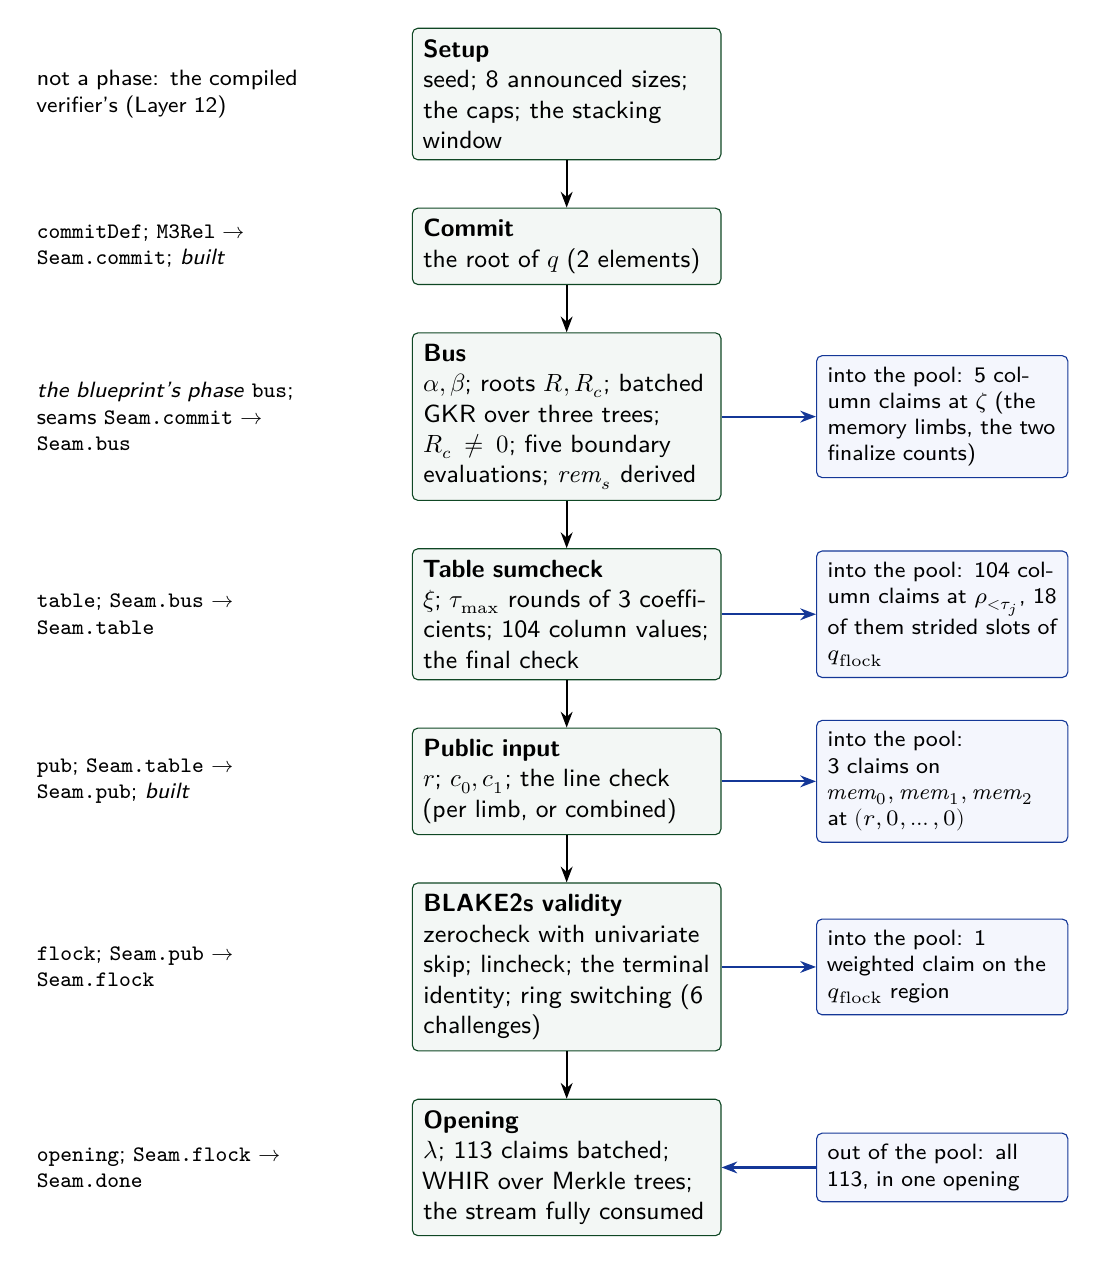
\begin{tikzpicture}[
  font=\small\sffamily, node distance=6mm,
  ph/.style={draw, rounded corners=2pt, fill=ok!5, draw=ok!70!black, text width=0.30\linewidth,
    align=left, inner sep=4pt},
  pool/.style={draw, rounded corners=2pt, fill=minor!5, draw=minor!70!black,
    text width=0.24\linewidth, align=left, inner sep=4pt, font=\footnotesize\sffamily},
  chal/.style={text width=0.30\linewidth, align=left, font=\footnotesize\sffamily},
  arr/.style={-{Stealth[length=2mm]}, thick}]
\node[ph] (setup) {\textbf{Setup} \\ seed; 8 announced sizes; the caps; the stacking window};
\node[ph, below=of setup] (commit) {\textbf{Commit} \\ the root of $q$ (2 elements)};
\node[ph, below=of commit] (bus) {\textbf{Bus} \\ $\alpha, \beta$; roots $R, R_c$; batched
  GKR over three trees; $R_c \neq 0$; five boundary evaluations; $\mathit{rem}_s$ derived};
\node[ph, below=of bus] (table) {\textbf{Table sumcheck} \\ $\xi$; $\tau_{\max}$ rounds of 3
  coefficients; 104 column values; the final check};
\node[ph, below=of table] (pub) {\textbf{Public input} \\ $r$; $c_0, c_1$; the line check
  (per limb, or combined)};
\node[ph, below=of pub] (flock) {\textbf{BLAKE2s validity} \\ zerocheck with univariate skip;
  lincheck; the terminal identity; ring switching (6 challenges)};
\node[ph, below=of flock] (open) {\textbf{Opening} \\ $\lambda$; 113 claims batched; WHIR
  over Merkle trees; the stream fully consumed};
\draw[arr] (setup) -- (commit); \draw[arr] (commit) -- (bus); \draw[arr] (bus) -- (table);
\draw[arr] (table) -- (pub); \draw[arr] (pub) -- (flock); \draw[arr] (flock) -- (open);
\node[pool, right=12mm of bus] (p1) {into the pool: 5 column claims at $\zeta$ (the memory
  limbs, the two finalize counts)};
\node[pool, right=12mm of table] (p2) {into the pool: 104 column claims at $\rho_{<\tau_j}$,
  18 of them strided slots of $\qflock$};
\node[pool, right=12mm of pub] (p3) {into the pool: 3 claims on $\mathit{mem}_0, \mathit{mem}_1,
  \mathit{mem}_2$ at $(r, 0, \dots, 0)$};
\node[pool, right=12mm of flock] (p4) {into the pool: 1 weighted claim on the $\qflock$
  region};
\node[pool, right=12mm of open] (p5) {out of the pool: all 113, in one opening};
\draw[arr, minor!70!black] (bus.east) -- (p1.west); \draw[arr, minor!70!black] (table.east) -- (p2.west);
\draw[arr, minor!70!black] (pub.east) -- (p3.west); \draw[arr, minor!70!black] (flock.east) -- (p4.west);
\draw[arr, minor!70!black] (p5.west) -- (open.east);
\node[chal, left=10mm of bus, anchor=east] {\emph{the blueprint's phase} \lean{bus}; seams
  \lean{Seam.commit} $\to$ \lean{Seam.bus}};
\node[chal, left=10mm of table, anchor=east] {\lean{table}; \lean{Seam.bus} $\to$
  \lean{Seam.table}};
\node[chal, left=10mm of pub, anchor=east] {\lean{pub}; \lean{Seam.table} $\to$
  \lean{Seam.pub}; \emph{built}};
\node[chal, left=10mm of flock, anchor=east] {\lean{flock}; \lean{Seam.pub} $\to$
  \lean{Seam.flock}};
\node[chal, left=10mm of open, anchor=east] {\lean{opening}; \lean{Seam.flock} $\to$
  \lean{Seam.done}};
\node[chal, left=10mm of commit, anchor=east] {\lean{commitDef}; \lean{M3Rel} $\to$
  \lean{Seam.commit}; \emph{built}};
\node[chal, left=10mm of setup, anchor=east] {not a phase: the compiled verifier's
  (Layer 12)};
\end{tikzpicture}
\caption{leanVM's proof system at the pin, as the deployed verifier runs it (centre), what each
phase adds to the claim pool (right), and the blueprint's phase and seams for it (left).}
\label{fig:phases}
\end{figure}

\section{What the blueprint makes of it}\label{sec:map-blueprint}

The blueprint models the protocol as a sequential composition of ArkLib \emph{oracle
reductions}, one per phase, in the ideal model where $q$ is an oracle and the challenges are
uniform (\cref{ch:libraries} introduces the vocabulary). It fixes, in the spine, what the
phases share: the abstract instance \lean{M3Instance}, the relation \lean{M3Holds}, the seam
relations, the interfaces \lean{Phase.Def}, \lean{Phase.Complete} and \lean{Phase.Security}, and
the composition with its two master theorems. It then specifies each phase (Layers 4 to 10),
the adaptor to leanISA (Layers 2 and 3), the compilation (Layers 11 and 12) and the target
theorem (Layer 13). \Cref{tab:map-where} says where each part is.

\begin{table}[h]
\centering\small
\begin{tabular}{@{}p{0.27\linewidth}p{0.30\linewidth}p{0.36\linewidth}@{}}
\toprule
Part & Blueprint & Code on \code{main} at \code{b435631} \\
\midrule
Fields, sampling, the oracle interface of $q$ & Layer 0 & \file{LeanerVM/Protocol/Field.lean}, \file{ToArkLib/Oracles.lean}; built \\
Hypercube tables, stacking, padding, the index and bytecode columns & Layer 1 & \file{ToCompPoly/*}, \file{Stack.lean}, \file{Padding.lean}, \file{ClaimWeights.lean}, \file{BlockClaims.lean}, \file{FixedColumns.lean}; built \\
The abstract instance, the relation, the seams, the interfaces, the composition, the master theorems & the section \enquote{The spine} & \file{Spine/\{Instance,Seams,Phase,Compose,Toy\}.lean}, \file{ToArkLib/\{Component,KnowledgeAppend,PassThrough,SendOracle,Refinement,GuardedVerdict,KeepOracles\}.lean}; built \\
Clean components as polynomials & Layer 2 & not built \\
The leanISA instance and the adaptor & Layer 3 & not built \\
The sumcheck and the batching component & Layer 4 & not built (an open pull request holds the honest round algebra) \\
Fingerprints, the grand product, GKR & Layer 5 & not built \\
The bus phase & Layer 6 & not built \\
The table sumcheck & Layer 7 & not built \\
The public-input phase & Layer 8 & \file{PublicInput.lean}; built, both halves proved \\
Flock and ring switching & Layer 9 & not built; owned by the Flock roadmap (issue \#3), which has not started \\
The claim pool and the opening & Layer 10 & not built \\
WHIR, Merkle trees, the parameters & Layer 11 & not built \\
Fiat--Shamir, the proof object, \lean{verify} & Layer 12 & not built \\
The target theorem & Layer 13 & not built \\
\bottomrule
\end{tabular}
\caption{Where each part of the proof system is specified and whether it is built.}
\label{tab:map-where}
\end{table}

Of the six phases, two are built: the commit phase, which is the spine's, and the public-input
phase. The four others, the generic components they rest on, the adaptor and the compilation
are specified only. The master theorems are therefore theorems about a \emph{bundle} of phases
supplied as a hypothesis; what they say, and what they leave to be trusted, is the subject of
\cref{ch:phases,ch:nonvacuity}.

\section{The reviewed revision and the one after it}\label{sec:map-revision}

The review's object is \code{main} at \code{b435631}. While the review was under way, the
owner upgraded \code{main} to Lean 4.34.1 (\code{144c5aa}, pull request \#61) and moved every
library pin: ArkLib to \code{7653a901}, CompPoly to \code{572f9973}, Clean to \code{42fe4b26},
VCVio to \code{a4232d08}. The leanVM pin did not move. The proof-system sources changed in
proofs and imports only (77 lines in, 76 out), so every statement this report discusses is the
same at both revisions; the two probability bridges of the spine were restated on VCVio's new
notation with the same relations and bounds. Two things did change in substance and are
recorded where they matter: ArkLib's new pin is the revision several dossiers examined as
\enquote{upstream}, and it lifts none of the admissions the blueprint's ledger names
(\cref{ch:libraries}); and CompPoly's $\K$ now gives natural-number literals their
characteristic-two meaning, $(2 : \K) = 0$, with encoded words written \lean{K.ofBits n}, so
that any probe or fixture using a literal other than $0$ or $1$ in $\K$ means something else at
the new pin (\cref{ch:probes}).

\chapter{The libraries, from scratch}\label{ch:libraries}

Every statement of the proof system unfolds to objects of four libraries. This chapter
introduces each object before anything is built on it: what it is, what it is for here, its
Lean text at the pin, and what a reader trusts in accepting it. The revision is named with each
snippet; where the upgrade of \code{main} to the new pins changed an object, both are given.
Readers who know Lean may skim; readers who do not should not skip the sections on VCVio and on
ArkLib's security notions, since the master theorems are statements in that vocabulary and
mean exactly what those definitions say.

\InputIfFileExists{sections/gen/lib-vcvio}{}{\emph{[fragment pending]}}

\InputIfFileExists{sections/gen/lib-comppoly}{}{\emph{[fragment pending]}}

\InputIfFileExists{sections/gen/lib-clean}{}{\emph{[fragment pending]}}

\InputIfFileExists{sections/gen/lib-lean}{}{\emph{[fragment pending]}}

\InputIfFileExists{sections/gen/lib-arklib-objects}{}{\emph{[fragment pending]}}

\label{sec:lib-security}
\InputIfFileExists{sections/gen/lib-arklib-security}{}{\emph{[fragment pending]}}

\label{sec:lib-pins}
\InputIfFileExists{sections/gen/lib-arklib-pins}{}{\emph{[fragment pending]}}

\label{sec:lib-layer0}
\InputIfFileExists{sections/gen/layer0-audit}{}{\emph{[fragment pending]}}

\chapter{Catalogue of the built code}\label{ch:catalogue}

Every public declaration of the proof system on \code{main} at \code{b435631}, grouped by file:
the structures with their fields, the definitions with their signatures (and their bodies where
the body is what a reader has to check), the theorem statements, the instances and the concrete
inhabitants. Each entry says what it means in plain language, what it depends on, and its
class: \textsf{load-bearing} (a master theorem's statement unfolds to it), \textsf{interface}
(a phase author or the adaptor must meet or consume it), \textsf{helper} (used inside proofs
only) or \textsf{test fixture}. Snippets are copied from the source at the revision reviewed.
The blueprint's per-layer sketches are compared with this catalogue in
\cref{sec:faith-conformance}; the audit surface it implies is measured in \cref{ch:auditability}.

\section{The spine}
\InputIfFileExists{sections/gen/catalogue-spine}{}{\emph{[fragment pending]}}

\section{The public-input phase}
\InputIfFileExists{sections/gen/catalogue-pubinput}{}{\emph{[fragment pending]}}

\section{Layer 1: tables, stacking, padding, claim weights, the fixed columns}
\InputIfFileExists{sections/gen/catalogue-layer1}{}{\emph{[fragment pending]}}

\section{The statements, read adversarially}\label{sec:cat-statements}
\InputIfFileExists{sections/gen/statements-spine}{}{\emph{[fragment pending]}}


\part{The analysis}
\chapter{The phases: what each proves, and how}\label{ch:phases}

This chapter gives, phase by phase, the design as the blueprint has it, the design as leanVM
has it, and the intuition behind the two proofs each phase owes: perfect completeness (an
honest prover always passes) and round-by-round knowledge soundness (an invariant on partial
transcripts that a cheating prover escapes only when a fresh challenge lands badly, with a
bound per challenge). Where the blueprint falls short of leanVM the finding is named and
detailed in \cref{ch:faithfulness}; where a definition cannot be met or says less than it
should, in \cref{ch:nonvacuity}. The vocabulary of the ideal model (oracle reduction,
knowledge state function, extractor) is introduced in \cref{ch:libraries}; the reader who has
that chapter in mind can read this one on its own.

\section{The commit phase}\label{sec:ph-commit}

The prover sends the stack $q$ as the one oracle message; the verifier keeps the statement and
exposes the message as the oracle. There is no challenge and no check. The phase is the spine's
own and both its halves are proved (\lean{commitComplete}, \lean{commitSecurity}). Its knowledge
state function says, before the message, that the candidate witness satisfies \lean{M3Holds}
and, after it, that the \emph{message} does; its extractor reads the message. Error zero is
right: there is no challenge to charge. In the deployed protocol the message is a Merkle root;
what a root must provide for the compiled protocol to inherit the oracle protocol's guarantee
is the subject of \cref{sec:ph-opening}.

\section{The bus phase}\label{sec:ph-bus}

\paragraph{What is proved.} That the multiset of tuples the tables push equals the multiset
they pull, on each of the three buses, and that every read count is nonzero. With the boundary
blocks (the initial and final machine state, the memory and bytecode seeds and finalizations)
counted in, balance is the whole of the memory and bytecode consistency of the execution.

\paragraph{How.} A fingerprint turns a 16-tuple $t$ into the scalar
$\beta + \sum_{i < 16} \eq(\alpha, i)\, t_i$ for random $\alpha \in \E^4$, $\beta \in \E$; two
multisets of at most $2^{\mu_{\mathrm{bus}}}$ tuples with different contents have different
products of fingerprints except with probability $4 \cdot 2^{\mu_{\mathrm{bus}}} / \abs{\E}$
(the specification's Theorem 5.1; each factor has total degree 4 in $(\alpha, \beta)$). The
product itself is proved by a grand-product argument: the leaves are the fingerprints (padded
with $1$), each layer of the tree holds pairwise products, and a GKR walk from the root
descends layer by layer, reducing a claim on a layer to a claim on the layer below by a
sumcheck; the three trees (push, pull, count) share every challenge and are batched by the
powers of a combiner $\lambda$. The prover states a single root $R$ for the push and pull
trees, so their equality needs no check, and a root $R_c$ for the count tree, which the
verifier requires to be nonzero. The walk ends with three claims on the leaf tables at one point
$\zeta$, which the leaf decomposition (the specification's equation (2) of §5.4) splits into a
public part the verifier computes, five boundary evaluations the prover sends, and the tables'
share, which the table sumcheck settles.

\paragraph{Completeness.} From \lean{M3Holds}: the constraints vanish, so the zerocheck claims
hold at every point; balance is a permutation, so the two products are one field element and
the honest prover has a single $R$ to send; every count is nonzero, so $R_c \neq 0$; the GKR's
honest messages pass every layer check (no inverse of a challenge is taken); the leaf
decomposition holds of the honest stack with the derived $\mathit{rem}_s$. This is perfect.

\paragraph{Knowledge soundness.} One state function for the whole phase, a conjunction:
before $(\alpha, \beta)$, \lean{M3Holds} of the oracle; after them, \enquote{the two products at
$(\alpha, \beta)$ are equal and $R_c$ is the true count product and every constraint vanishes};
from then on the GKR's own invariant (\enquote{the current layer claims are the true values})
together with the zerocheck conjunct \enquote{every constraint's extension, restricted to the
coordinates of $\zeta$ drawn so far, is identically zero}. A challenge flips a false state
to true with probability at most: $4 \cdot 2^{\mu_{\mathrm{bus}}} / \abs{\E}$ for
$(\alpha, \beta)$; $2 / \abs{\E}$ for a combiner (the batching polynomial has degree 2);
$4 / \abs{\E}$ for a round challenge (the cofactor has degree 4); $1 / \abs{\E}$ for a
combination challenge; and $0$ for the last, unused combiner. The zerocheck conjunct adds
nothing: on a coordinate of $\zeta$ it flips with probability at most $1 / \abs{\E}$, once for
all constraints (a nonzero multilinear restricted at one more variable becomes zero for at most
one value of that variable), and a conjunction escapes with the larger of the two
probabilities, not their sum. The blueprint's three different accounts of this charge, and its
GKR of the wrong degree, are the findings of \cref{sec:faith-bus}.

\paragraph{Where the blueprint falls short.} The GKR layer sumcheck it specifies has degree 5
and is not the deployed one (\emph{normalized} cofactor of degree 4, no equality factor in the
layer check); it draws one combiner fewer than the deployed verifier; its generic GKR takes the
leaf tables as oracles, which the spine's one-oracle phases cannot supply without ArkLib's
admitted context lifting; and the zerocheck conjunct, which changes on the GKR's own
challenges, cannot be framed around a GKR that knows nothing of the constraints. The admissible
sizes it equates with leanISA's caps leave out the stacking window and the rate window that the
deployed verifier checks. None of this touches the spine as built: the real bus phase's output
is expressible as a \lean{BusOut}, and its completeness and knowledge soundness against the
spine's two seams can hold (\cref{sec:faith-bus}).

\section{The table sumcheck}\label{sec:ph-table}

\paragraph{What is proved.} That every constraint of every opcode table vanishes on every row
(for leanVM at the pin, the two identities of the JUMP table; the other tables have none), and
that each table's bus forms sum, over its rows, to the share $\mathit{rem}_s$ the bus phase
derived for it. The second is what ties the committed columns to the bus trees: the trees were
built by the prover, and only this sumcheck says that they were built from the columns.

\paragraph{How.} One sumcheck over $\tau_{\max}$ variables, the highest bound first, with each
table joining at the round where its height is reached and padded below it by the product of
the variables it lacks (so that its sum is unchanged). The summand batches the constraints and
the three bus forms by the powers of $\xi$, with $\eq(\zeta_{< \tau_j}, \cdot)$ as the weight
of table $j$: the constraint terms contribute zero to the target and the bus terms contribute
$\sum_s \xi^{2 + s}\, \mathit{rem}_s$, which the verifier computes, so no target is ever sent.
A round message is a cubic (the equality factor times a degree-2 term) of which three
coefficients travel; the verifier derives the fourth from the running claim. At the end the
prover sends every column's value at the sumcheck's point and the verifier recomputes the
summand.

\paragraph{Completeness.} Immediate from the input seam: the zerocheck claims are true, the bus
forms sum to their values, the honest round polynomials pass, the honest column values
reproduce the summand. No inverse of a challenge is taken.

\paragraph{Knowledge soundness.} Before $\xi$: every claim is true. After $\xi$: the batched
claim $\sum_c \xi^c\, \delta_c = 0$ where $\delta_c$ is claim $c$'s error; a nonzero polynomial
of degree at most $k - 1$ in $\xi$ has at most $k - 1$ roots, so the error on $\xi$ is
$(k - 1) / \abs{\E}$, which is $(B + 2) / \abs{\E}$ for $B$ constraints and three sides. Each
round: if the running claim is false, the prover's cubic differs from the true one and they
agree at most at three points, $3 / \abs{\E}$. After the last message: the verifier accepts and
every column claim holds, so the recomputed summand is the true summand at the point and the
running claim was true. The escape from \enquote{the zerocheck claims hold at $\zeta$} to
\enquote{the constraints vanish on the cube} belongs to the bus phase, where $\zeta$ was drawn
(above); it is not charged here.

\paragraph{Where the blueprint falls short.} Not in the numbers, which are right and tight,
but in the seam it consumes. \lean{Seam.bus} as built admits statements that the deployed table
sumcheck cannot serve: any number of linear claims (so the error on $\xi$ is unbounded over the
seam), terms of one table at unrelated points, terms on any table of the instance, and a degree
clause on the statement alone, which forces the verifier to check degrees, a check leanVM does
not make. Completeness and knowledge soundness are owed on all of them. The blueprint also
leaves open which tables the sumcheck ranges over: its leanISA instance makes the six shared
columns tables of the instance, and read literally its table sumcheck then has at least sixteen
rounds where leanVM has as few as three (\cref{sec:faith-table}). And its oracle protocol sends
four coefficients and checks the round identity, where the deployed verifier reads three and
derives the fourth; the lemma relating the two is not stated.

\section{The public-input phase}\label{sec:ph-pub}

\paragraph{What is proved.} That cells 0 and 1 of the three memory limbs hold the two public
words: for the two low limbs, the words' limbs; for the top limb, zero.

\paragraph{How.} The verifier draws $r \in \E$ and considers the line through cells 0 and 1 of
a column: $\widetilde{c}(r, 0, \dots, 0) = (1 - r)\, c(0) + r\, c(1)$, where $-1 = 1$ in
characteristic 2. The prover sends the values $c_0, c_1$ it claims for the two low limbs on
that line. The specification checks each against the line through the public words' limbs;
the deployed verifiers check the single equation $c_0 + y\, c_1 = (1 + r)\, w_0 + r\, w_1$ in
$\E$, which the two per-limb equations imply and which does not imply them. Three claims are
then pooled: the two low limbs at the values sent and the top limb at $0$, for which nothing is
sent.

\paragraph{Completeness.} If the lines hold, the honest values pass either check and every
pooled claim is a true evaluation. Perfect.

\paragraph{Knowledge soundness.} A wrong stack (a cell of a limb differing from the public
word's) makes the pooled claim on that limb a nonzero polynomial of degree one in $r$, true at
one challenge at most: error $1 / \abs{\E}$, whatever the number of lines and for either
check. For the deployed check the argument runs through the independence of $1, y, y^2$ over
$\K$: if the three pooled claims hold of a $\K$-valued memory and the combined equation holds
at two distinct challenges, the cells are the limbs of the public words and the top limbs are
zero. This is proved in Lean by the review (\cref{ch:probes}).

\paragraph{Where the phase as built falls short.} It follows the specification, so its theorem
is about a verifier that none of the three executable verifiers runs. And it pools the values
it \emph{computes} from the statement rather than the values \emph{sent}: on the accepting path
they agree, but the consequence is that the check on the prover's message is not load-bearing
for any theorem of the phase: a verifier that reads the message and ignores it has the same
completeness and the same knowledge soundness at the same error. The requirement that a missing
check leave a theorem unprovable is therefore not met by this phase as designed, and cannot be;
pooling the values sent, as the deployed verifiers do, restores it (\cref{sec:faith-pub},
\cref{ch:drift}). The top-limb claim exists because the leanISA instance lists a third public
line; nothing in the phase or the spine forces that line, and what catches its absence is the
adaptor's theorem, not built (\cref{ch:drift}).

\section{BLAKE2s validity and ring switching}\label{sec:ph-flock}

\paragraph{What is proved.} That the bits packed into the region $\qflock$ of the stack satisfy,
block by block, the R1CS of the BLAKE2s compression with the constant position of every block
equal to $1$; the eighteen value limbs each BLAKE2S table row carries are strided slots of that
region and are opened with every other point claim.

\paragraph{How.} Flock is a zerocheck over the R1CS's rows, with the first six variables
skipped univariately (the prover sends the summand on a coset of 64 points), followed by a
lincheck that reduces the three matrix products to one evaluation of the bit witness at a
point, with a single terminal identity the verifier checks. Ring switching then turns the 64
resulting claims on the bit polynomials $Q_i$ (bit $i$ of every word) at one point into a
weighted claim on the packed column: for a random $\F_2$-linear map $\Phi$ built from six
challenges, $\sum_u \Phi(\eq(r, u))\, \qflock(u) = \sum_i x^i\, \Phi(s_i)$, whose weight the
verifier evaluates in closed form. Neither step commits anything: the only oracle is $q$.

\paragraph{Completeness.} Perfect, for the honest prover that sends the coefficients of the
true round polynomials: the verifier derives the untransmitted coefficient by a multiplication
and takes no inverse. The \emph{deployed} Rust prover is not that prover: it derives $G(0)$
through $(1 + r_{\mathrm{eq}})^{-1}$, whose value at $r_{\mathrm{eq}} = 1$ is $0$ by the
field's convention, and at that challenge emits a proof its own verifier rejects. The
blueprint's acceptance test 20 attributes this inverse to the protocol and files it under a
soundness error; both are wrong (\cref{sec:faith-flock}).

\paragraph{Knowledge soundness.} The specification's Annex C accounts
$(4 k_{\mathrm{batch}} + 163) / \abs{\E}$ for the reduction, which the review re-derived term by
term from the Rust's parameters, and Annex A accounts below $2^{32} / \abs{\E}$ for ring
switching (a nonzero polynomial of total degree below $2^{32}$ in the six challenges). Both are
errors for a fixed committed polynomial; after compilation the list-decoding regime multiplies
them by the list size (\cref{sec:ph-opening}).

\paragraph{Where the blueprint falls short.} Its Layer 9 makes the eighteen limb claims an
\emph{input} of Flock and one weighted claim its only output, dropping the limb claims; with
leanVM's verifier, which reads no claim, that interface has knowledge error one. The spine's
slot, which keeps the column claims and adds the weighted one, is right. The slot map of the
limbs is placed inside the Flock interface while the instance's layout needs it. And a Flock
phase cannot be written over an abstract instance at all, since the instance offers it only an
opaque predicate \lean{aux}; the review proposes a small structure that names the region, the
number of compressions and what \lean{aux} says of them (\cref{sec:faith-flock}). Today, with
the only built instance having \lean{aux} trivially true, a Flock phase that checks nothing is
knowledge sound at error zero (\cref{ch:probes}): the master theorems constrain the Flock
verifier exactly as much as the instance's predicate does.

\section{The opening and the compilation}\label{sec:ph-opening}

\emph{This section is completed from the dossier on the opening, WHIR, Merkle trees and
Fiat--Shamir, which is being finished as this draft is written.} What is already established:
the specification's opening is one batching challenge followed by one inner-product opening,
with no separate reduction sumcheck, whereas the blueprint's oracle protocol runs a sumcheck
reducing the batched weighted claim to an evaluation and then queries the oracle once; the
oracle interface of the stack in Layer 0 is an evaluation oracle, and an inner-product oracle,
the idealization of the specification's Definition 3.13, would make the opening phase
\enquote{$\lambda$, then one query} with leanVM's transcript. The compiled error the blueprint
sketches lacks the hash-collision term, the list-size factor of a list-binding commitment and
any account of grinding; the assumed Fiat--Shamir and BCS interfaces are stated for
constructions that are not leanVM's single BLAKE2s map (\cref{sec:faith-opening}).

\chapter{The proof obligations, as a hierarchy}\label{ch:obligations}

The tree of everything that must be proved for the proof system's target theorem to hold,
from the root down to the library facts the leaves rest on, with the status of every node at
\code{b435631} and the nodes the review found wrong, missing or unprovable. The two existing
outlines, the obligation map of \file{docs/architecture.md} and the blueprint's table of holes,
are validated against it at the end. The tree was drawn by a review agent from the blueprint,
the dossiers and the sources; its Markdown form is \file{dossiers/obligations.md} on the review
branch.
\ifobligationsready\InputIfFileExists{sections/gen/obligations}{}{}\else\emph{[The obligations tree is being typeset; it is inserted here when it lands.]}\fi

\chapter{The trusted base}\label{ch:tcb}

What a reader has to accept without a proof in this repository, in order to believe the
master theorems and the theorems the blueprint builds on them. The accounting is in layers,
from the kernel outward; each entry says what is trusted, why, and whether the blueprint names
it. \Cref{ch:auditability} measures the part of it that is leanerVM's own definitions.

\section{Lean and its three axioms}

Every theorem of the proof system, the port of the composition theorem included, closes on
\lean{propext}, \lean{Classical.choice} and \lean{Quot.sound} and on nothing else, at both pins
(\cref{ch:probes}); the repository's validation rejects \lean{sorryAx} across its two
namespaces with a planted-axiom control, and forbids \lean{native_decide}, whose trust would be
the compiler's rather than the kernel's. A \texttt{\#guard} trusts the compiled evaluator; a
\lean{decide} the kernel's reduction (\cref{ch:libraries}). The kernel and the elaborator are
trusted as every Lean development trusts them.

\section{The libraries' definitions}

The statements unfold to definitions of four libraries, which a reader must accept as meaning
what they should: ArkLib's protocol specifications, oracle reductions, run semantics,
completeness, knowledge state functions, extractors and round-by-round knowledge soundness;
VCVio's oracle computations as distributions, its probabilities and its uniform sampler; and
CompPoly's tables, polynomials and the two fields. Clean's objects enter through
\lean{SatisfiedBy}, on the other side of the adaptor. \Cref{ch:libraries} introduces each and
records what the review checked of it: the fields are leanVM's bit for bit, the samplers are
uniform by the class's law, the oracle interface of the stack answers the extension in the
specification's bit order, and ArkLib's notion of knowledge soundness is non-vacuous. Two
caveats stay: ArkLib's definition of a knowledge state function deliberately differs from the
literature's (its own docstring says so), and its existential notion of round-by-round
knowledge soundness is soundness, since the extractor may be a classical choice; the spine's
named form is knowledge with the extractor read.

\section{Theorems the libraries admit, on which the chain will rest}

None of leanerVM's theorems depends on an admitted theorem today; the chain the blueprint
plans does, at both pins:
\begin{itemize}
\item the implication from round-by-round to plain knowledge soundness, which gives the master
  theorem its prover-level reading (a bound on the success of a cheating prover rather than a
  property of transcripts); its conclusion is existential in the extractor;
\item the security of the Fiat--Shamir and Merkle (BCS) compilations, which ArkLib does not
  state (its BCS transform is commented out, its commitment extractability has \lean{False} for
  a body, its Fiat--Shamir completeness is admitted and stated for a constant challenge
  oracle);
\item the coding-theory theorem behind WHIR's soundness, mutual correlated agreement up to the
  Johnson bound, which ArkLib admits and which in the literature is a single-version preprint
  with a sketched proof;
\item ring switching, whose leaves ArkLib admits, and which is in any case another protocol
  than leanVM's.
\end{itemize}
The blueprint's ledger names the first and the second and the third; it describes the fourth
as a missing profile, which it is not (\cref{sec:faith-flock}). The new pin lifts none of
them.

\section{The interfaces the blueprint assumes}

Four structures are taken as arguments of the non-interactive theorems and one of the
adaptor: the Flock phase with its security and its error, the Fiat--Shamir and BCS security
statements, the coding-theory theorem, and the Flock witness generator. Each is meant to be a
structure whose fields are theorems another roadmap or an upstream library owes. What the
review found: none exists in Lean; the Flock interface as sketched has knowledge error one
against leanVM's verifier and cannot be stated over an abstract instance; the Fiat--Shamir and
BCS interfaces are stated for constructions that are not leanVM's single BLAKE2s map, and the
Fiat--Shamir one, as \enquote{the query bound times the largest round error}, cannot certify
leanVM's 128 bits, which the query rounds reach only through grinding
(\cref{sec:faith-opening}). A structure taken as a hypothesis is trusted exactly when it is
inhabited by a theorem; until then a theorem that takes it says nothing, and the repository's
own rule against uninhabited load-bearing types applies.

\section{The instance for leanISA}

The oracle protocol is stated over an abstract instance; leanVM enters through the leanISA
instance, which is data: the tables' shapes, the constraint polynomials and flush tuples read
off Clean's components, the count columns, the boundary blocks with their known columns (the
index column and the program's bytecode columns), the layout of the stack with its
tie-breaking order, the three public lines, the Flock region and its predicate. Two theorems
are meant to pin that data to the arithmetization (\lean{satisfiedBy_witnessOf} and
\lean{m3Holds_stackOf}) and one fixture to the deployed layout; none exists. What the review
established about the data's shape (\cref{ch:faithfulness}): the instance is not
\lean{Ensemble.toM3} of the eight tables, and the adaptor's soundness direction works only
because the seed, finalization and state blocks are boundary blocks with known columns built
from the same program the witness is rebuilt from; the layout has no reader for the eighteen
limb columns; the admissibility predicate must contain the stacking and rate windows; the
polynomial bridge of Layer 2 is noncomputable at the pin. Until the adaptor is built, the
instance is trusted in full, and no theorem on \code{main} says that its relation is inhabited.

\section{Hypotheses of the chain, and who discharges each}

\begin{longtable}{@{}p{0.30\linewidth}p{0.36\linewidth}p{0.30\linewidth}@{}}
\toprule
Hypothesis & Kind & Discharged by \\
\midrule
\endhead
\lean{Phases.Complete}, \lean{Phases.Security} & the phases' proofs & four of five phases unbuilt; the built ones prove theirs \\
a bound on \lean{piopError} & missing from the spine & nothing; to be fixed in the spine \\
\lean{s.Admissible prog} (sizes within the caps and the windows) & a property of announced public data & the compiled verifier's setup checks; today, nothing \\
\lean{WellFormedBytecode prog} (the sentinel is not a jump; fill blocks) & a decidable property of the public program & leanISA's constraint-soundness theorem takes it; the blueprint's target theorem omits it, and nobody is told to check it \\
the public words' top limbs are zero & a property of the public input & by the type of \lean{PublicInput}; in the deployed verifier, a rejection at setup that the blueprint does not mention \\
resource conditions on the execution (a memory that fits in $2^{28}$ committed cells, heights within the caps) & a property of the trace & nothing; the blueprint's completeness target is false without them \\
\lean{HasFillBlocks prog} & a property of the program & leanISA's constraint-completeness theorem takes it \\
the Flock witness generator and its lemma & another roadmap's & the Flock roadmap, which has not started \\
the Fiat--Shamir, BCS and coding-theory interfaces & upstream theorems & ArkLib, which states none of them today \\
BLAKE2s as a random oracle & a heuristic, not a theorem & nothing; the blueprint does not state it as a hypothesis \\
the Rust verifier is \lean{verify} & an implementation correspondence & a fixture of Rust-produced proofs with mutations; evidence, not proof \\
\bottomrule
\end{longtable}

\section{Outside Lean}

Three things no theorem of the repository can reach. The random-oracle heuristic: every
non-interactive guarantee is a statement about a verifier with a random oracle, and the
deployed verifier hashes with BLAKE2s; the known attacks on this gap do not reach leanVM's
structure, and the guarantee is classical (\cref{ch:options}). The implementation: the Rust verifier
verifier is what Ethereum would run, and it is tied to the Lean verifier by tests only; the
review found one check on which they already differ in strength. The hardware, the compiler and the
toolchain, as for every Lean development.

\section{What the blueprint says of its trusted surface}

Its convention \emph{Trusted surface} asks that every trusted definition fit on one screen,
cite its source line, and appear in its interface list; its interface list closes with
\enquote{everything not listed is a proof, a helper, or a test}. The review found fourteen
load-bearing declarations of the spine not listed, 198 of the proof system's 333 public
declarations absent from it, and several listed names that do not exist
(\cref{ch:faithfulness}); its \enquote{assumed interfaces a reviewer must know} are the right
four, with the qualifications above; and its headline's account of what is proved without
hypotheses (\enquote{everything about the oracle protocol}) overstates what is on \code{main}
by the four unbuilt phases, the missing error bound and the instance.


\part{The audit}
\chapter{Faithfulness}\label{ch:faithfulness}

For each phase of the oracle protocol and for the compilation, this chapter sets the blueprint
side by side with the specification and with the Rust and Python verifiers at the pin: the
transcript (who sends what, in which order, which challenge is drawn after which message),
the checks the verifier makes (in \cref{ch:drift}, where they serve the check-by-check
enumeration), the disagreements between the three sources, and the findings, each classified
as an error of the blueprint, a deliberate deviation with the theorem it owes, or a deviation
an upstream library forces. The tables and the findings were written by the review's agents
from the sources, then checked citation by citation by independent agents; the corrections
are marked in place. leanVM's revision is \code{a386121f} throughout, read from git after the
checkout moved (\cref{ch:brief}).

\section{How to read the tables}

A transcript row is one step of the deployed verifier: a prover message with its size, a
verifier challenge, a computation or a check, with the three sources' lines. A disagreement is
a place where the specification, the Rust and the Python do not say the same thing; where the
two verifiers agree and the specification is silent or differs, the blueprint follows the
verifiers and the report says so. A finding names what the blueprint gets wrong or leaves out,
with its evidence and the change proposed.

\section{The spine}\label{sec:faith-spine}

The spine is not a phase, but the seams and the error are where the phases' faithfulness is
decided, and three of the review's findings on it belong here: the bus seam admits statements
the deployed table sumcheck cannot serve (\cref{sec:faith-table}); the error of the composed
protocol is the phases' own declaration, so that the knowledge-soundness theorem constrains
nothing until a bound is stated (\cref{sec:nv-hypotheses}); and the blueprint states the
master theorems, the phases' statement types and the opening's objects two or three times
differently, with the code implementing the spine's version every time
(\cref{sec:faith-conformance}). The findings on the spine's code are collected in
\cref{sec:faith-code}.

\section{The setup, the commitment and the bus}\label{sec:faith-bus}

\InputIfFileExists{sections/gen/transcript-bus}{}{\emph{[transcript fragment pending]}}
\InputIfFileExists{sections/gen/disagreements-bus}{}{}
\InputIfFileExists{sections/gen/findings-bus}{}{\emph{[findings fragment pending]}}

\paragraph{The review's verdict on the GKR round error.} Two dossiers charged a radix-4 round
differently: $4/\abs{\E}$ (the bus dossier, from the deployed cofactor of degree 4) and
$5/\abs{\E}$ (the table-sumcheck dossier, taking the blueprint's number when it argued that the
zerocheck conjunct adds nothing). The orchestrator read the verifier loop
(\file{crates/lean_vm/src/gkr.rs:399-413}): the round message is five coefficients of which
four travel, the first derived through the equality factor from the running claim, and the
layer's final check has no equality factor. A wrong running claim makes the prover's cofactor
differ from the true one, both of degree 4, so the next claim is right at four challenges at
most: $4/\abs{\E}$ is the deployed error, the blueprint's $5/\abs{\E}$ is a loose bound that
also describes a different, non-normalized protocol, and the second dossier's argument stands
with $4/\abs{\E}$ in place of $5/\abs{\E}$.

\section{The table sumcheck and the public input}\label{sec:faith-table}\label{sec:faith-pub}

\InputIfFileExists{sections/gen/transcript-table-pub}{}{\emph{[transcript fragment pending]}}
\InputIfFileExists{sections/gen/disagreements-table-pub}{}{}
\InputIfFileExists{sections/gen/findings-table-pub}{}{\emph{[findings fragment pending]}}

\section{BLAKE2s validity and ring switching}\label{sec:faith-flock}

\InputIfFileExists{sections/gen/transcript-flock-ring}{}{\emph{[transcript fragment pending]}}
\InputIfFileExists{sections/gen/disagreements-flock-ring}{}{}
\InputIfFileExists{sections/gen/findings-flock-ring}{}{\emph{[findings fragment pending]}}

\section{The opening and the compilation}\label{sec:faith-opening}

\InputIfFileExists{sections/gen/transcript-opening}{}{\emph{[The dossier on the opening,
WHIR, Merkle trees and Fiat--Shamir is being finished; its transcript, disagreements and
findings are inserted here when it lands.]}}
\InputIfFileExists{sections/gen/disagreements-opening}{}{}
\InputIfFileExists{sections/gen/findings-opening}{}{}

\section{The adaptor and the boundary with leanISA}\label{sec:faith-adaptor}

\InputIfFileExists{sections/gen/findings-boundary}{}{\emph{[The findings of the boundary
dossier are inserted here when their LaTeX fragment lands; the nine major ones are summarised
in \cref{ch:tcb}.]}}

\section{The code as built: the spine, Layer 1, the public-input phase}\label{sec:faith-code}

\InputIfFileExists{sections/gen/conformance}{}{\emph{[conformance fragment pending]}}
\label{sec:faith-conformance}
\InputIfFileExists{sections/gen/findings-code}{}{\emph{[findings fragment pending]}}

\section{The libraries and Layer 0}\label{sec:faith-libraries}

\InputIfFileExists{sections/gen/findings-libraries}{}{\emph{[findings fragment pending]}}

\chapter{Non-vacuity}\label{ch:nonvacuity}

A definition is non-vacuous when it is inhabited by the object leanVM intends and refuted by
the near misses; a theorem, when its hypotheses can be met by the real protocol and not only by
a trivial one, and when what it concludes is not already true of everything. This chapter
records what the review established by probe, in Lean, against \code{main} at \code{b435631},
and what it established on paper. The probes are reproduced in \cref{ch:probes}; the rule of the
review was that a conclusion resting on a probe names it.

\section{The relation and the seams}\label{sec:nv-relation}

\paragraph{\lean{M3Holds}.} On the toy instance the honest stack satisfies it, and for each of
the four checkable clauses a stack fails that clause alone: the repository's own tests do this
(\file{tests/LeanerVMTests/Protocol/Spine.lean}). The review added the cases those tests lack
(probe \code{P2Relation}): a tuple pushed twice and pulled once fails \lean{Balanced}, and a
tuple pushed twice and never pulled fails it too, which a balance summed in the field would
accept; the side filter and the row ranges of \lean{tuples} were exercised on instances built
for the purpose. Clause by clause against the pinned specification, \lean{M3Holds} is the
relation the bus, the table sumcheck, the public-input check and Flock together establish
(\cref{ch:faithfulness}); the review found no clause wrong.

\paragraph{The seams.} Each seam was inhabited and refuted per conjunct (probe \code{P3aSeams});
the zerocheck escape, a constraint violated on the cube whose extension vanishes at the point
$(1)$, was exhibited on a stack \code{badConstraint} to show that the bus seam's claims can hold
of a stack outside \lean{M3Holds}, which is what the error of the bus phase pays for.
\lean{Seam.done} is \lean{True}, so the last law of a knowledge state function reads
\enquote{if the verifier accepts then the state is true} (probe \code{NonVacuity}); this is
what an output relation carrying nothing should give.

\paragraph{What the seams admit beyond leanVM.} \lean{Seam.bus} admits statements the deployed
bus phase never emits and the deployed table sumcheck cannot serve: a statement true of an
honest stack yet outside the seam by its degree clause alone; a linear claim with two terms of
one table at two points; a thousand copies of a true claim (probes \code{SeamBusShape},
\code{SeamBusMember}). This is not a vacuity of the seam but a burden on the phase that
consumes it, developed in \cref{sec:faith-table}.

\section{The hypotheses of the master theorems}\label{sec:nv-hypotheses}

The two master theorems take a bundle of phases with their proofs, \lean{Phases.Complete} and
\lean{Phases.Security}. Whether these can be met, and by what, is the question.

\paragraph{They can be met by the real phases.} For the bus phase, the table sumcheck and the
public-input phase the review worked out, on paper, a knowledge state function and per-challenge
errors that meet \lean{Phase.Security} against the spine's seams (\cref{ch:phases}); the
public-input phase's is built and proved. For Flock, perfect completeness is attainable by the
honest prover of the specification, and the blueprint's belief that it is not (its acceptance
test 20) is mistaken (\cref{sec:faith-flock}). For the table sumcheck the answer is
\enquote{yes, by a generalized phase with guards leanVM does not have}, which is the finding of
\cref{sec:faith-table}. For the opening, see \cref{sec:faith-opening}.

\paragraph{They can also be met by protocols that are not leanVM's.} Three constructions,
two of them machine-checked:
\begin{enumerate}
\item \textbf{Phases that check nothing, at declared error one.} A phase that draws one
  challenge, ignores it, makes no query and outputs a function of its input statement is
  perfectly complete whenever that function carries one seam into the next, and is
  round-by-round knowledge sound against \emph{any} two seams at the error it declares for its
  challenge, namely $1$. Five of them inhabit \lean{Phases.Security\ I} for every instance
  $I$; both master theorems hold of the bundle; the composed error is $1$ at each of its five
  challenges (probe \code{P4Junk}, standard axioms only). The knowledge-soundness master theorem
  therefore has content only together with a bound on \lean{piopError}, and the spine states
  none: \lean{piopError\ P} is \lean{P.toDef.err}, whatever the phases declare. The blueprint's
  \lean{piopError_le} (Layer 10) is stated over sizes the spine's \lean{piopError} does not take.
  This is the review's first major finding on the spine (\cref{sec:faith-spine}); the proposed
  repair is a closed-form error fixed by the spine from the instance and demanded of each phase.
\item \textbf{Phases that read the whole stack.} In the ideal model the verifier may query
  $\widetilde{q}$ at every point of the cube, and neither ArkLib nor the spine counts queries;
  \lean{M3Holds} is decidable. So a phase with no round whose verifier reads the $2^{\mu}$ cells
  and decides the input seam itself is perfectly complete and knowledge sound at error zero.
  Five of them inhabit \lean{Phases.Security\ I} for every $I$ with \lean{piopError} $= 0$. On
  paper (two dossiers reach it independently); a probe was designed and not run.
\item \textbf{A verifier that always rejects} is knowledge sound at error zero and is excluded
  only because \lean{Security} extends \lean{Complete}: on an instance whose relation is empty
  (below) the exclusion is void.
\end{enumerate}
Conversely, the five pass-through phases of the repository's tests, which inhabit
\lean{Phases.Complete}, have \emph{no} \lean{Phases.Security}: the type is empty (probe
\code{P5PassThrough}, theorem \code{no\_security}), where the test's docstring only asserts it.

\paragraph{What this means.} The master theorems are composition theorems. They pin the
phases to leanVM's by nothing in their statement; what does is outside the spine and, today,
outside the repository: a bound on the error (item 1), the phases' definitions being leanVM's,
which only the compiled verifier's refinement theorem and the fixture of a Rust-produced proof
can tie down (item 2), and review of each phase's definition against the specification. The
report's recommendation is to move the first into the spine and to say the other two plainly
in the blueprint's headline (\cref{ch:options}).

\section{The instance}\label{sec:nv-instance}

The relation is stated over an abstract instance, and an instance can be wrong in ways the
spine does not exclude. A \lean{Layout} that reads every column from cells $0$ and $1$
satisfies the reading law (probe \code{P2Relation}, \code{toyAlias}); on it the three columns
are one, \lean{M3Holds} asks for incompatible things, and the relation is empty for every stack
and statement (exhaustive on the cells, the general case on paper). The master theorems hold of
that instance: completeness is vacuous, and knowledge soundness says that every accepting
prover was lucky. The reading law also determines \lean{read} from \lean{extend} (a cube point's
extension is the cell), so \lean{read} is redundant data and the only freedom of an instance is
\lean{extend}. A wrong \lean{extend} costs completeness and faithfulness, never the soundness of
the Lean chain: the adaptor's theorem from \lean{M3Holds} to \lean{SatisfiedBy}, if proved of
such an instance, still gives the chain to the semantics. Who rules such instances out is the
adaptor's completeness theorems and the transcription of the layout with the compiled verifier's
fixture, none of which is built; until then, no statement on \code{main} says that the relation
of any instance other than the toy is inhabited.

The same holds of the instance's other fields: \lean{aux} is an arbitrary predicate, and on the
only built instance it is \lean{True}, so a Flock phase with no message, no challenge and no
check is knowledge sound at error zero (probe \code{NoCheckFlock}); \lean{publicLines} is a
list, and an instance with two lines instead of three has every theorem of the spine and of the
public-input phase (\cref{ch:drift}); \lean{Layout.comap}, by which the adaptor is to name the
blocks, accepts a renaming that is not one-to-one, so columns can alias.

\section{The error bound}\label{sec:nv-error}

Beyond item 1 above: the errors the blueprint charges to the bus phase, the table sumcheck and
the public-input phase are correct and tight where they are stated, and the review's
round-by-round arguments give the state functions that attain them (\cref{ch:phases}). Two
errors are not tight: the zerocheck escape, which costs $\tau_{\max} / \abs{\E}$ once and
nothing in a conjunctive state function, is charged per constraint and placed on the wrong
challenges; and the GKR round error is $4 / \abs{\E}$, not $5 / \abs{\E}$. Whether the sum
means something at leanVM's parameters is settled in \cref{sec:faith-opening}: the interactive
sum does (about $2^{32.3} / \abs{\E}$ under the stacking window, within the blueprint's
$2^{40} / \abs{\E}$), but the non-interactive
bound the blueprint sketches leaves out three things that decide whether leanVM reaches the
128 bits it claims.

\section{The extractor}\label{sec:nv-extractor}

Every extractor in the repository is a compiled definition: nothing along the chain from
\lean{piopExtractor} to the commit phase's is marked \lean{noncomputable}, and the three of them
run (probes \code{P1Axioms}, \code{Extractors}). \lean{#print\ axioms} says nothing about this:
it reports the three standard axioms for computable definitions whose proofs use classical
lemmas, and the earlier review's use of it as evidence of computability was a misreading.

Two things are less than the blueprint says. First, \enquote{the extractor's column $q$
satisfies \lean{M3Holds}} names no definition of the repository: the composed extractor's
\lean{extractOut} returns the stack only when every phase has no round; with the repository's
own public-input phase in the bundle, the statement of the test that \enquote{the extractor
returns the committed stack} is ill-typed, because \lean{extractOut} then lives in that phase's
last intermediate witness type, \lean{Unit} (probe \code{P3cExtractor}, an expected failure
recorded). The stack is what the composed extractor returns at round $0$ through its
\lean{extractMid} at the commit round, and there it is the transcript's first message whatever
it is handed. No function \enquote{the stack extracted from a full transcript} is defined.
Second, ArkLib's extractor type accepts an extractor that chooses a witness by classical choice,
and such an extractor is \enquote{knowledge sound at error zero} for any relation whose
language the verifier decides (probe \code{Extractors}): ArkLib's existential notion of
round-by-round knowledge soundness is soundness, and the named form the spine uses is knowledge
only with the named extractor read. A phase's \lean{Security} could carry a classical extractor
without anything in the repository noticing; it would not matter, because from the commit phase
on the witnesses are \lean{Unit} and the stack comes from the commit phase's extractor alone,
which is the spine's and reads the message. The design \enquote{the oracle is the witness}
excludes the risk that acceptance test 24 guards against; the test does not.

\section{The public-input phase}\label{sec:nv-pubinput}

The phase is built and its two theorems are proved; the question is what they exclude. The
answer, machine-checked (probe \code{ProbeAnyCheck}, theorem \code{securityG}): nothing about
the check. For every function the prover may use to compute its message and every Boolean check
that the honest message passes, the phase with that check has a \lean{Phase.Security} against
the same seams at the same error $1 / \abs{\E}$. Instances proved: no check and no message; no
check and a message of forty-two zeros; a check with the two cells swapped, with a prover that
sends the swapped values. The reason is one line of the definition: \lean{pooled} takes its
values from the statement, not from the message, and the proof of knowledge soundness never
mentions \lean{check}. What the theorems do exclude, each refuted in Lean with no extractor,
state function or error below one able to repair it (theorem \code{not\_rbr}, which denies
ArkLib's existential notion): a verifier that pools the prover's values without checking them;
one that checks only the first value and pools the prover's values; one that does not pool the
claim of a line whose value is not sent. The earlier review's statement that each of five wrong
verifiers breaks a stated theorem was true of the build it read and is false of the code as
merged: its own compression (pooling the lines' values, its own first compression) removed the
dependence, and the status file still repeats the claim. The consequence for the requirement
that a missing check leave a theorem unprovable is drawn in \cref{ch:drift}; the repair, pooling
the values sent, is proposed in \cref{sec:faith-pub}.

\section{The notion itself}\label{sec:nv-notion}

ArkLib's round-by-round knowledge soundness is not trivially satisfiable: a verifier that
accepts everything has no knowledge state function for a non-trivial relation with no rounds,
and with one challenge it is not knowledge sound at error zero whatever the extractor; every
verifier is knowledge sound at error one (probe \code{NonVacuity}). Its plain reading, that an
accepting transcript either extracts a witness or contains a challenge that fell in the bad set
of its prefix, is machine-checked at the transcript level (probe \code{PlainReading}); the
step from there to a bound on a prover's success is ArkLib's admitted implication from
round-by-round to plain knowledge soundness, at both pins (\cref{ch:libraries}).

\section{The blueprint's acceptance tests}\label{sec:nv-acceptance}

The blueprint names twenty-eight acceptance tests, each a reading that compiles and is wrong
with the witness that rejects it. For each, whether the witness exists on \code{main} and the
review's verdict.
\InputIfFileExists{sections/gen/acceptance-tests}{}{\emph{[table pending]}}

\section{What was not established}\label{sec:nv-open}

The read-everything phase (item 2 of \cref{sec:nv-hypotheses}) is on paper. The emptiness of
the aliased instance's relation is exhaustive on the cells and on paper in general. Of the
mutation probes of the public-input phase, two were never written (the deployed check with the
prover's values pooled, the wrong point) and rest on paper; two (the wrong check with the
honest prover unchanged, the extra check) ran at the new pins and refuted completeness as
predicted, while their unchanged knowledge-soundness proof failed at the state function like
every other mutation's (\cref{ch:probes}).

\chapter{Auditability}\label{ch:auditability}

The audit surface of a theorem is the set of declarations its statement unfolds to: what a
reader must read, and trust to mean what it says, before the theorem tells them anything. This
chapter separates those declarations from the helpers, measures them, and proposes what can be
removed without changing any statement's meaning. Faithfulness and non-vacuity come first; the
proposals here are for after the statements are right.

\section{What is load-bearing}\label{sec:aud-loadbearing}

For the two master theorems the load-bearing declarations are, transitively: the theorems'
statements (\lean{piop_perfectCompleteness}, \lean{piop_rbrKnowledgeSoundness}); the
composition (\lean{leanVmPiop}, \lean{leanVmVerifier}, \lean{piopError}, \lean{piopExtractor},
\lean{Phases}, \lean{Phases.toDef}, \lean{Phases.Complete}, \lean{Phases.Security}, and the
commit phase's four declarations); the component interfaces (\lean{Component.Def},
\lean{Complete}, \lean{Security}, their \lean{append}, the two ported composition
declarations); the seams (\lean{Seam.of} and the six seams, the four claim structures with
their \lean{Holds}, the four output structures, \lean{theStack}); the instance
(\lean{M3Instance} with its fields, \lean{Shape}, \lean{Layout}, \lean{Coord},
\lean{BoundaryBlock}, \lean{PublicLine}, the readers \lean{column}, \lean{row},
\lean{coordCell}, \lean{tuples}, the four clauses, \lean{M3Holds}, \lean{M3Rel},
\lean{TheOracle}); and Layer 0's oracle interface of the stack with the field and sampling
instances. Below them sit the library definitions they unfold to, which \cref{ch:libraries}
introduces: ArkLib's protocol specifications, oracle reductions, completeness, knowledge state
functions, extractors and round-by-round knowledge soundness; VCVio's computations and
probabilities; CompPoly's tables, polynomials and fields.

Measured at \code{b435631} (probe \code{P6Surface}; the tables are in \cref{sec:aud-tables}):
the completeness theorem unfolds to 70 declarations and 217 lines of statements (382 with
docstrings); the knowledge-soundness theorem in its existential form to 76 declarations and
248 lines (432); in the named form the spine states, to 100 declarations and 354 lines (612).
Layer 1 has 143 public declarations, of which 20 are load-bearing and 41 are interfaces; an
auditor of the master theorems reads none of them today, 17 definitions (61 lines) become
trusted once the adaptor is built and about 8 more (22 lines) once the executable verifier is.
The public-input phase adds its verifier, its check, its pool and its line identity.

\section{What is not, and whether it leaks}\label{sec:aud-helpers}

A helper lemma cannot enlarge the trusted surface of a theorem it helps to prove: the kernel
checks the proof, and what the proof used does not change what the statement says. Two things
can leak nonetheless, and were checked. An \emph{axiom} used by a helper propagates to every
theorem that uses it: every theorem of the proof system, the port of the composition included,
closes on the kernel's three standard axioms and on nothing else (\lean{#print\ axioms},
probe \code{AxiomsLeanerVM}, re-run at the new pins in \cref{ch:probes}), and the repository's
validation rejects \lean{sorryAx} across both namespaces with a planted-axiom control. An
\emph{instance} used by a statement (a decidability instance, a sampler, an oracle interface)
is part of the statement's meaning: the sampler instances are uniform by VCVio's class law, the
diamond on the sampler of $\K$ resolves to the same term by \lean{rfl}, and the oracle
interface of the stack answers the extension at the point in the specification's bit order
(\cref{ch:libraries}). No helper was found to enlarge the trusted surface.

\section{Proposals to reduce the surface}\label{sec:aud-proposals}

Each proposal names what is removed, what it costs and whether a statement changes. None
changes the meaning of a master theorem; the first two are also faithfulness repairs and are
argued in \cref{ch:faithfulness}.

\begin{enumerate}
\item \textbf{Fix the error in the spine.} Replace the phases' declared \lean{err} by a closed
  form \lean{piopError\ I} computed from the instance, and demand each phase's knowledge
  soundness at it. Removes a field from \lean{Component.Def} and the possibility of item 1 of
  \cref{sec:nv-hypotheses}; adds one definition to the spine. Changes the statement of the
  knowledge-soundness theorem, for the better: it then says something.
\item \textbf{Give the bus seam leanVM's shape.} Replace \lean{BusOut}'s list of linear claims
  by one point, the forms per side and table with the degree bound in their type, three totals
  and the column claims. Removes \lean{LinearClaim}, \lean{VirtualTerm}, the degree conjunct of
  \lean{Seam.bus} and the guards a generalized table sumcheck would need; adds three small
  types. Changes \lean{Seam.bus} and the two phases around it.
\item \textbf{Derive \lean{read} from \lean{extend}.} The reading law determines it
  (\cref{sec:nv-instance}); \lean{Layout} then has one field of data and one law, and an
  instance cannot state a \lean{read} that disagrees with its \lean{extend}. Costs one
  definition and a lemma; changes no statement's meaning.
\item \textbf{Delete \lean{outputPure}.} It is derivable for every component over the empty
  shared oracle (probe \code{P6Surface}, \code{outputPure\_of\_def}; ArkLib has the instance at
  the pin). Removes a field of \lean{Component.Complete} and one obligation per phase.
\item \textbf{Separate the guard from completeness.} A base structure with the guarded form
  only, extended by \lean{Complete} and by \lean{Security}, so that knowledge soundness no
  longer presupposes perfect completeness (\cref{sec:faith-flock}). Costs one structure;
  changes no theorem's meaning; changes what an author of a phase must prove first.
\item \textbf{Drop \lean{Weight.mle} from the seam.} The evaluator the verifier runs is the
  opening phase's business, not the seam's; the seam needs the cube values and the value.
  Removes a field and a law from \lean{Weight}; the closed form of the ring-switching weight
  stays owed to whoever builds the opening.
\item \textbf{Merge \lean{TableOut} and \lean{PubOut}.} Both are a list of column claims; one
  structure with two uses. Removes one structure; changes the type of the public-input phase's
  slot, not its meaning.
\item \textbf{Move the error out of \lean{Component.Def}.} With item 1 the field is gone; even
  without it, keeping a real number in the definition makes every phase with a challenge
  \lean{noncomputable}, so that neither the verifier nor the extractor compiles when reached
  through the phase (probe \code{ExtractorsExpectedFailure}). The executable verifier of Layer 12
  is meant to read the phases' definitions.
\item \textbf{Delete \lean{BlockClaims.lean}.} It has no consumer, and the earlier review found
  that no phase can use it over an abstract instance. Removes about a dozen declarations.
\item \textbf{Say which tables the sumcheck ranges over}, as a decidable predicate on the
  instance's tables derived from its constraints, flushes and counts (\cref{sec:faith-table}).
  Adds one definition; removes a whole class of instances the table sumcheck would otherwise be
  owed on.
\item \textbf{Name the Flock region in the instance} (a column, a log-count, a height fact and
  what \lean{aux} says of it) instead of the opaque predicate alone (\cref{sec:faith-flock}).
  Adds one small structure; makes the Flock phase statable over an abstract instance.
\item \textbf{Read the existential theorem first.} \lean{piop_rbrKnowledgeSoundness_exists}
  unfolds to 24 fewer declarations than the named form; a reader should start there, then read
  the named form for the extractor.
\end{enumerate}

With items 2, 4, 6, 7 and 9 applied the review estimates the named knowledge-soundness form at
about 80 declarations and 290 lines of statements; the estimate is not a measurement.

\section{The measured tables}\label{sec:aud-tables}

\InputIfFileExists{sections/gen/surface}{}{\emph{The measured tables of the audit surface, per
file and per class, are produced from the spine and Layer 1 dossiers and are inserted here.}}


\part{What to do}
\chapter{Options, limitations and boundaries}\label{ch:options}

For each thing the review found, the options are to fix the blueprint, to keep it with the
reason recorded and a theorem owed, or to refactor it; this chapter gives the review's
recommendation with the cost of each, then the general trade-off between specifying leanVM
exactly as deployed and specifying a variant that is easier to audit, then what cannot be
reproduced today and what it waits on, and finally what the proof system hands over to, and
requires of, the rest of the end-to-end verification. The register of findings
(\cref{sec:reg}) numbers each finding \code{R1}, \code{R2}, \ldots; the appendix of proposed
changes (\cref{ch:changes}) gives the text of each change.

\section{Recommendations, in priority order}\label{sec:opt-recommendations}

\begin{enumerate}
\item \textbf{Fix the error in the spine} (\code{R5}). Define \texttt{piopError I} in closed
  form from the instance's sizes and demand each phase's knowledge soundness at it. Cost: one
  definition and a change of one field; every phase built later pays the bound. Without it the
  soundness theorem constrains nothing. The alternative, a bound as a field of
  \lean{Phases.Security}, keeps the phases' freedom to declare and is weaker; not recommended.
\item \textbf{Give the stack an inner-product oracle} (\code{R18}). The specification's
  commitment is an inner-product scheme; its idealization answers weighted sums. The opening
  phase becomes \enquote{$\lambda$, then one weighted query}, with the deployed transcript, and
  WHIR replaces the whole opening phase. Cost: Layer 0's interface, the opening phase and
  Layers 11 and 12 as sketched; nothing built breaks. The alternative, keeping the evaluation
  oracle and the extra sumcheck and owing a theorem that relates the two protocols, is a
  transcript leanVM does not have and a theorem nobody has stated; not recommended. A third,
  ending the oracle protocol at the Flock seam and treating the opening as part of the
  compilation, is acceptable but moves the batching error out of the oracle protocol.
\item \textbf{Give the bus seam leanVM's shape and name the sumcheck's tables}
  (\code{R2}, \code{R11}). One point, forms per side and table with the degree bound in the
  type, three totals, the column claims; a decidable predicate for the tables the sumcheck
  ranges over. Cost: the seam and the two phases around it; the removal of the guards a
  generalized table sumcheck would otherwise need. The alternative, keeping the general seam
  with a generalized verifier and proving the guards dead in the composition, is more code and
  a verifier that is not leanVM's; not recommended. The bus phase's side of the seam is right
  either way (\code{R3}).
\item \textbf{Build the public-input phase of the deployed verifiers} (\code{R12},
  \code{R13}). The combined check, with the values sent pooled; its key lemma is proved. Keep
  the specification's phase as a reference and report the discrepancy of §8.2 to leanVM as an
  ambiguity (both are sound). Cost: one phase, on the pattern of the built one. The alternative,
  keeping only the specification's phase, leaves the master theorem about a verifier nobody
  runs and a check that no theorem needs.
\item \textbf{Make the Flock phase statable and its interface faithful} (\code{R14},
  \code{R15}, \code{R16}, \code{R17}). A small structure in the instance naming the region, the
  log-count and what the predicate says; the slot map of the limbs as parameters, not as a
  field of the Flock interface; Layer 9's interface replaced by the spine's slot; the honest
  prover the mathematical one; acceptance test 20 rewritten; the Rust prover's defect at
  $r_{\mathrm{eq}} = 1$ reported to leanVM. Cost: text, one structure, and a request to the
  Flock roadmap. Whether \lean{Component.Complete} should carry an error (\code{R4}) is then
  a choice: not needed for faithfulness, useful as insurance; the review recommends separating
  the guard from completeness so that knowledge soundness no longer presupposes it, and leaving
  completeness perfect.
\item \textbf{Describe the GKR as deployed} (\code{R7}, \code{R9}, \code{R10}). The
  normalized layer sumcheck of degree 4, four coefficients on the wire, error $4/\abs{\E}$; a
  combiner after every layer, the last unused; a GKR component over a context with the leaf
  tables derived from the stack and the zerocheck conjunct riding along, or a monolithic bus
  phase. Cost: Layers 4 to 6 as sketched. The alternative, ArkLib's context lifting, is admitted
  at both pins.
\item \textbf{Restate the adaptor} (\code{R30} to \code{R33}, \code{R35}). The instance built
  from the tables' components and from boundary blocks with known columns, never
  \lean{Ensemble.toM3} of the eight tables; a bridge lemma for the boundary blocks; a computable
  polynomial bridge; admissibility with the stacking and rate windows and no
  \lean{logInvRate} in the witness's sizes; a reducible instance; the strided reader of the limb
  columns as a Layer 1 lemma and a Layer 3 reader. Cost: Layers 1 to 3 as sketched.
\item \textbf{Restate the non-interactive theorems} (\code{R20} to \code{R29}). An adversary
  with a query budget against a random oracle standing for the compression and for the
  multi-block hash of the Merkle leaves, a straight-line
  extractor that reads leaves off the query log, list decodes and selects, adversary-chosen
  sizes inside one protocol family, the program bound by its hash, the well-formedness of the
  program and the resource bounds as hypotheses, and the random-oracle heuristic as a named
  non-formal step; the error with the hash term, the list-size factor and grinding; completeness
  of the honest prover whenever its grind returns. The assumed interfaces restated for leanVM's
  constructions (one BLAKE2s map for the chain, the Merkle nodes and the grinding), or replaced
  by a plan to prove the chain lemma and the role-separation lemma; the list-binding
  compilation stated as the theorem it is. Cost: Layers 11 to 13 rewritten; the target theorem
  of \file{docs/architecture.md} with them.
\item \textbf{Decide the framework} (\code{R34}). ArkLib now calls \lean{OracleReduction}
  legacy and its typed successor has no knowledge notion; the composition the spine ports is
  still admitted upstream and its pull request still open. Stay on the legacy framework with
  the local port, and record the decision and its retirement condition, or plan the migration.
  The review recommends staying, since nothing upstream is ready to receive the spine, and
  records the trigger to revisit: a knowledge notion and a composition theorem for it in the
  typed framework (\cref{ch:arklib-landscape}).
\item \textbf{Rewrite the upstream ledger on what ArkLib has} (\cref{ch:arklib-landscape}).
  Consume the typed sumcheck for the plain case only, through an adaptor from the spine's
  oracle reductions; write the leanVM-shaped sumchecks and every knowledge leaf locally, and
  drop the plan to contribute the classical leaf, which is false as stated; consume VCVio's
  Merkle trees; state the proved Johnson-range bound as the coding-theory interface's candidate
  and check its constant against the specification's budget; define the inner-product oracle
  locally, since nothing upstream has or plans it.
\item \textbf{Consolidate the documentation} (\code{R36} to \code{R38} and the minor rows).
  The blueprint as the one specification, its per-layer sketches rewritten on the spine's
  types, the hole comment folded into it, the status and the tracker as pointers, one
  vocabulary, the codes replaced by names or indexed once (\cref{ch:documentation}).
\end{enumerate}

\section{Exactly as deployed, or easier to audit?}\label{sec:opt-tradeoff}

The review's rule of thumb, from what it found: \emph{the oracle protocol models the checks
of the deployed verifier; the specification is the source of the arguments.} Where the two
agree, there is no choice. Where they differ, three cases arose. The public-input check: the
specification's per-limb check is easier to reason about and the deployed combined check is
what runs; modelling the specification's produced a theorem about a verifier nobody runs and a
check that no theorem needs, so the deployed one should be modelled and the specification
amended. The Flock prover's inverse: a defect of the implementation's prover, not of the
protocol, so the Lean honest prover is the specification's and the implementation is told. The
Python verifier's acceptance of nonzero absent lanes: soundness-neutral, recorded, not
modelled. The general lesson is that an auditable variant is acceptable only where it accepts
\emph{no more} than the deployed verifier and its relation to the deployed one is a theorem
somebody states; a variant that accepts less (the per-limb check) makes the master theorem
silent about the deployed verifier's extra acceptances, which is where a deployment's risk is.

Two deliberate deviations the blueprint has are right and should stay with their reasons
written: the oracle protocol's messages are whole objects where the wire carries an encoding
(the round polynomial with one coefficient derived), owing the transport lemma the review
states; and the relation is polynomial rather than \enquote{an execution exists}, with the
adaptor as the one place the semantics is met.

\section{What cannot be reproduced today}\label{sec:opt-upstream}

\begin{itemize}
\item Clean's bus balance over $\K$ is unsatisfiable, not merely unsound: leanISA's
  \lean{BalancedPair} stands in until Clean's directed, integer-counted balance lands and the
  pin reaches it (\cref{ch:libraries}).
\item ArkLib admits the composition of knowledge soundness (ported locally), the implications
  from round-by-round to plain knowledge soundness and soundness, the sumcheck's round-by-round
  leaf, context lifting, and the coding-theory theorem; it states no Fiat--Shamir or Merkle
  security; its ring switching is another protocol. None of this moved with the new pin. The
  chain to the target theorem waits on the implications and on Fiat--Shamir, and the review
  recommends stating the assumed interfaces for leanVM's constructions now, so that what is
  waited for is at least written down.
\item Lean's kernel cannot decide the fields' arithmetic fast: probes over $\K$ and $\E$ are
  \texttt{\#guard}s on tiny instances, and a numeral's meaning in $\K$ changed with the new pin.
\item No published theorem covers Fiat--Shamir with proof of work for a multi-round protocol;
  leanVM's query rounds reach 128 bits only with it. The blueprint should say what security
  level its non-interactive theorem can certify and what remains a claim of the parameter
  analysis.
\end{itemize}

\section{What to report to leanVM}\label{sec:opt-upstream-report}

The review changes nothing upstream and posts nothing; the matters below are what the owner
may report, each with its source lines and its register row.
\InputIfFileExists{sections/gen/report-upstream}{}{\emph{[list pending]}}

\section{The boundaries}\label{sec:opt-boundaries}

\paragraph{What the proof system requires of leanISA.} The relation \lean{SatisfiedBy} as it
stands, with its \lean{Caps}, its integer-counted balance, its fixed-column conjuncts and its
public-word conjunct whose top limb is zero by type; the constraint-soundness theorem with its
hypothesis \lean{WellFormedBytecode}, which the target theorem must carry; a resource condition
on valid executions, without which completeness is false; and the two requests the blueprint
already makes (power-of-two heights, bus data per channel), both met.

\paragraph{What it requires of the Flock roadmap.} A predicate on a packed column (the R1CS
with the constant position), a phase at the spine's seams with perfect completeness for the
specification's honest prover and knowledge soundness at the accounted error, the witness
generator with its lemma, the constants and the slot map transcribed from the Rust verifier (they are
not in the specification), and the ring-switching weight's closed form. The roadmap has not
started; the compiled verifier's fixture cannot pass before its definition exists.

\paragraph{What it hands over.} To the arithmetization: knowledge of \lean{M3Holds} of the
leanISA instance at the proof system's error, carried by the adaptor to \lean{SatisfiedBy}. To
recursion: the compiled verifier with its fixed-claim settlement as the seam, and the extracted
witness the recursion target needs, which the target theorem as sketched drops. To Ethereum: a
verifier whose every check has a theorem behind it or a named reason why not, which is what
\cref{ch:drift} sets out to make enforceable.

\chapter{The documentation: one source of truth}\label{ch:documentation}

The blueprint, the status, the tracker with its hole comment, the review handoffs and the
lists of findings overlap, use different terms for the same things, and disagree with the
repository. This chapter inventories which document says what, lists the contradictions with
evidence, proposes one owner per kind of fact with the others pointing to it, one vocabulary,
and the treatment of the letter codes; \cref{ch:tracker} holds the resulting texts, ready to
apply, and \cref{ch:codeindex} the index of every code. Nothing here has been applied: the
review changes no document and posts nothing.

\section{Which document says what}
\InputIfFileExists{sections/gen/docs-inventory}{}{\emph{[fragment pending]}}

\section{Contradictions and stale statements}
\InputIfFileExists{sections/gen/docs-contradictions}{}{\emph{[fragment pending]}}

\section{Vocabulary}
\InputIfFileExists{sections/gen/docs-vocabulary}{}{\emph{[fragment pending]}}

\section{The letter codes}
\InputIfFileExists{sections/gen/docs-codes}{}{\emph{[fragment pending]}}

\section{The proposal}\label{sec:docs-proposal}
\InputIfFileExists{sections/gen/docs-proposal}{}{\emph{[fragment pending]}}

\section{Findings on the documentation}
\InputIfFileExists{sections/gen/findings-docs}{}{\emph{[fragment pending]}}

\chapter{Keeping the Lean verifier from drifting away from the deployed one}\label{ch:drift}

The requirement, stated by the owner: a verifier that omits a check leanVM makes, or makes a
weaker one, must have no proof of knowledge soundness; a verifier that makes a wrong check, or
one leanVM does not make, must have no proof of completeness. The theorems, not the tests, are
to keep leanerVM faithful. This chapter says where that holds today, where it does not and why,
and what would make it hold as the work proceeds and the pin moves.

\section{Where a weakening can hide}\label{sec:drift-hiding}

The chain from \lean{verify} to the semantics (\cref{fig:chain}) has five places where a
missing or wrong check could go unnoticed by the master theorems. For each, the review says
whether it occurs today.

\paragraph{The relation weakened in step with the verifier.} The relation is
\lean{M3Holds I input q}, and \lean{I} is data: its \lean{publicLines}, its \lean{aux}, its
\lean{counts}, its \lean{boundary}, its \lean{constraints} and \lean{flushes}, its
\lean{layout}. A verifier that omits the claim on the top memory limb, together with an
instance that lists two public lines instead of three, is knowledge sound: every theorem of the
spine and of the public-input phase holds of the two-line instance. A Flock verifier that checks
nothing, together with an instance whose \lean{aux} is \lean{True}, is knowledge sound at error
zero (probe \code{NoCheckFlock}). An instance whose layout aliases columns has an empty
relation and both master theorems (probe \code{P2Relation}). \emph{This occurs.} It is the
price of stating the protocol over an abstract instance: the instance is where leanVM's
relation enters, and the oracle protocol's theorems cannot check the instance. What catches a
weakened instance is the adaptor's soundness theorem, \lean{satisfiedBy_witnessOf}, whose
conclusion \lean{SatisfiedBy} does not weaken with the instance: a two-line instance leaves its
public-word conjunct unprovable (\lean{SatisfiedBy.word0\_eq} has the top limb zero by the type
of \lean{PublicInput}); a trivial \lean{aux} leaves \lean{Blake2sRowsValid} unprovable; an
aliasing layout leaves the completeness theorem \lean{m3Holds_stackOf} unprovable. Behind the
adaptor, \lean{constraintSoundness} anchors \lean{SatisfiedBy} to \lean{ValidExecution}. None of
these three theorems is built. \textbf{Until the adaptor is built, the master theorems
constrain the instance by nothing, and a weakening of the instance is caught by no theorem on
\code{main}.}

\paragraph{A property supplied as a hypothesis that nothing discharges.} The master theorems
take \lean{Phases.Complete} and \lean{Phases.Security} as hypotheses; four of the five phases
are unbuilt, so the hypotheses are undischarged. Worse, \lean{Phases.Security} can be
discharged by phases that check nothing at declared error one (probe \code{P4Junk}): the error
is the phases' own field. \emph{This occurs}, and it is the finding that most changes how the
soundness theorem should be read (\cref{sec:nv-hypotheses}). The repair is to fix the error in
the spine, so that a phase can only meet its slot by earning the bound.

\paragraph{A check behind an assumed interface.} Flock, ring switching, WHIR's soundness, the
Merkle compilation and Fiat--Shamir are consumed as interfaces. Today none exists in Lean; when
they exist, a check the deployed verifier makes inside one of them (the lincheck's terminal
identity; the Merkle path check; the grinding check) is load-bearing only for the interface's
own theorem, which another roadmap or an upstream library owes. \emph{This occurs by design},
and the report accepts it on two conditions: that each interface is a structure whose fields are
theorems with named owners and no inhabitant in the repository until they are proved (the
repository's own rule against uninhabited load-bearing types then flags them), and that the
interfaces are stated for leanVM's constructions, which the Fiat--Shamir and BCS ones today are
not (\cref{sec:faith-opening}).

\paragraph{A property lost between the abstract instance and leanISA's, or in the adaptor.}
The instance for leanISA does not exist; the adaptor does not exist. What the review found is
that the blueprint's sketch of them cannot be written as it stands (the admissibility predicate,
the strided reader of the limb columns, the Flock predicate, the fit of the layout) and that
the sketch's \lean{witnessOf} builds parts of the witness from the program, which is sound only
if balance is then proved of the mixed witness (\cref{ch:faithfulness}). \emph{Cannot occur
yet}, since nothing is there to lose it; the report's recommendations for Layer 3 are where it
must be prevented.

\paragraph{A check present in the oracle verifier and absent from the compiled one, or in Lean
and absent from Rust.} The compiled verifier does not exist. Between Lean and Rust the review
found one check Lean makes in a stricter form than the deployed verifiers (the per-limb
public-input check, where they check one combined equation), one that the deployed verifiers make and Lean's oracle protocol cannot (the proof of
work), and three format checks the blueprint does not list (canonical encodings of the sizes
and of the root, the stream fully consumed). \emph{This occurs} at the public-input phase
today, and would occur at the compilation as planned.

\section{The public-input phase, as the test case}\label{sec:drift-pubinput}

The owner's own example was the top lane of the two public words. Following it to its anchor:

\begin{enumerate}
\item In the deployed verifier, two things enforce it: the statement-level rejection of a
  public word with a nonzero top limb at setup (\file{cpu/mod.rs:141-143}), and the pooled claim
  that the top memory limb is zero at $(r, 0, \dots, 0)$, for which no scalar is sent.
\item In Lean, the first is enforced by the type: leanISA's \lean{PublicInput} is four lanes of
  $\K$, so a nonzero top limb is not writable. The second is the third public line of the
  leanISA instance, which the blueprint specifies and which nothing on \code{main} states.
\item The phase pools the third claim because the instance lists a third line. Drop the line
  and every theorem of the spine and of the phase still holds (\cref{sec:nv-pubinput}). The
  master theorems do not catch it.
\item The adaptor's theorem \lean{satisfiedBy_witnessOf} would: \lean{SatisfiedBy} requires
  the memory cells $0$ and $1$, as three-limb values, to be the public words, whose top limb is
  zero by type. Without the third line the top limb of the extracted memory is unconstrained
  and the conjunct is unprovable. Behind it, \lean{constraintSoundness} carries the conjunct to
  the semantics.
\item So the answer to the owner's question is: \textbf{the master theorems do not catch it;
  the adaptor's soundness theorem does, once it exists; the blueprint's acceptance test 10 is a
  test on the pool, not a theorem.} The chain is anchored, but its anchor is two unbuilt
  theorems away from the oracle protocol.
\end{enumerate}

The same phase gave a second, harder lesson. Its check on the prover's message is not
load-bearing for any theorem, because the verifier pools the values it computes rather than the
values it received (\cref{sec:nv-pubinput}). The requirement cannot be met for that check by
any theorem about the phase as designed, since omitting the check yields a sound verifier: a
verifier that ignores the message and pools the statement's values is right to do so. What
makes the check load-bearing is the design of the deployed verifiers, which pool the values
\emph{sent}: with \lean{pooledFrom} in place of \lean{pooled} the omission and the weakening are
refuted by Lean theorems and a wrong check breaks completeness for every prover (probes
\code{Probe2TrustProver}, \code{Probe3b}, \code{Probe7a}). The rule this gives is general:
\emph{a check is load-bearing only if the verifier commits to what it checked.} A phase that
recomputes what the prover sent makes the message, and its check, decorative.

\section{The checks of the deployed verifier, one by one}\label{sec:drift-checks}

For every check the deployed verifier makes at the pin, the tables below give where it is in
the three sources, what it protects, the concrete cheating prover or witness a verifier
without it would accept, and, where a phase is built, the Lean check and the theorem that
makes it necessary. They are the review's enumeration from the specification and from the
rejection paths of the Rust and Python verifiers; the setup's checks and the format checks are
included, since the compiled verifier must make them and the blueprint does not list them.

\InputIfFileExists{sections/gen/checks-bus}{}{\emph{[The checks of the setup, the commitment
and the bus phase: fragment pending.]}}
\InputIfFileExists{sections/gen/checks-table-pub}{}{\emph{[The checks of the table sumcheck
and the public-input phase: fragment pending.]}}
\InputIfFileExists{sections/gen/checks-flock-ring}{}{\emph{[The checks of the BLAKE2s validity
phase and ring switching: fragment pending.]}}
\ifopeningready\InputIfFileExists{sections/gen/checks-opening}{}{}\else\emph{[The checks of the opening and of the compiled verifier: fragment pending.]}\fi

Three checks stand out because no planned theorem makes them load-bearing: the proof of work
(grinding), the canonical encodings, and the consumption of the stream. The first is a soundness
check in the non-interactive setting only, and no published theorem covers Fiat--Shamir with
proof of work for a multi-round protocol; the other two are format checks whose omission lets
\lean{verify} accept streams the deployed verifier rejects. All three need a mutation test in
the compiled verifier's fixture (\cref{sec:drift-mechanisms}).

\section{What keeps it true}\label{sec:drift-mechanisms}

\paragraph{Stated once, so that it cannot drift.} The relation, the seams and the error: the
first two are the spine's already; the error is to be (\cref{sec:aud-proposals}). With the
error fixed by the spine, a phase that declares less than it earns does not typecheck against
its slot.

\paragraph{What each phase delivers before it lands.} For each check of the phase's verifier,
a \emph{refutation}: a Lean theorem that the verifier without that check has no round-by-round
knowledge soundness against the seams at any error below one, whatever the extractor and the
state function; and for each check the deployed verifier does not make, a theorem that the
verifier with it is not perfectly complete. The public-input phase's audit gives the two
generic lemmas this needs (\code{not\_rbr} and \code{not\_perfectCompleteness},
\cref{ch:probes}); they belong in \file{ToArkLib/}. A mutation whose omission cannot be
refuted is a check the verifier does not rely on, and the phase's design should be revised
until it does (the rule of \cref{sec:drift-pubinput}). These refutations are tests under
\file{tests/}, run by \code{lake test}, and a phase's pull request lists them.

\paragraph{What ties the Lean verifier to the deployed one.} The compiled verifier's refinement
theorem ties \lean{verify} to the oracle protocol by definition; only a fixture ties either to
the Rust. The fixture is a proof produced by the pinned Rust prover, accepted by \lean{verify}
under \lean{\#guard}, with a mutation per check: each of the checks of \cref{sec:drift-checks}
gets a mutated proof that the deployed verifier rejects and that \lean{verify} must reject too.
The blueprint's six mutations become as many as there are checks. Reverse tests, transcripts
the specification rejects run through the Rust and Python verifiers, are how the per-limb
public-input divergence would have been found by a test rather than by a reader; the review
recommends them for every check whose statement in the specification differs from the code.

\paragraph{What is examined again when the pin moves.} The leanVM pin: every check of
\cref{sec:drift-checks} against the new verifier's rejection paths, the message and challenge
counts of every phase, the layouts and their tie-breaking orders, the constants of Flock and
of Fiat--Shamir, the parameter tables. The library pins: the admitted theorems the ledger names
(this upgrade lifted none), the notation of the probability bridges (this upgrade changed it),
the meaning of numerals in $\K$ (this upgrade changed it), and every acceptance test that
\lean{decide}s a numeral.

\paragraph{What the repository's validation can enforce.} Today it enforces the axiom
closure, the absence of \lean{sorry}, the layer DAG and the documentation index. It can also
enforce: the wall (a rule in \file{scripts/check-layers.sh} listing the modules allowed to
import the arithmetization, which today would flag \file{Protocol/Basic.lean}); the presence,
for every built phase, of a refutation test per check (a script that reads the phase's checks
from a manifest and asserts a test per entry); the fixture and its mutations, once the
compiled verifier exists; and, at a pin move, a script that re-derives the message and
challenge counts of every phase from its \lean{Def} and compares them with counts dumped from
the Rust prover. What it cannot enforce is that a phase's definition is leanVM's: that rests
on review against the specification, which is why this report's tables of the transcript
exist.


\appendix
\part{Appendices}
\chapter{Proposed changes to the blueprint}\label{ch:changes}

One entry per change, ordered by where in the blueprint it applies, each pointing to the
finding that carries its full text: the passage as it stands, the passage as proposed, and
the reason. The changes to the status file, the tracker and the other documents are in
\cref{ch:tracker}; the changes to the code are in the second table. Nothing here has been
applied.
\ifchangesready\InputIfFileExists{sections/gen/changes}{}{}\else\emph{[fragment pending]}\fi

\chapter{The probes}\label{ch:probes}

Every Lean or Python probe a conclusion of this report rests on, with its source, the command
that ran it, its recorded output and the revision it ran at. Probes ran against \code{main} at
\code{b435631} with the old pins unless marked otherwise; those re-run after the upgrade are
marked with their outcome at the new pins. A probe marked \enquote{written, not run} supports no
conclusion beyond the paper argument it accompanies.

\section{The spine, the public-input phase, Layer 1}
\InputIfFileExists{sections/gen/probes-code}{}{\emph{[fragment pending]}}

\section{The boundary with leanISA}
\InputIfFileExists{sections/gen/probes-boundary}{}{\emph{[fragment pending]}}

\section{Re-runs at the new pins}
\InputIfFileExists{sections/gen/probes-rerun}{}{\emph{[The re-run of the written-but-not-run
probes and of those whose numerals changed meaning, at the new pins, is inserted here when
it completes.]}}

\chapter{Index of the letter codes}\label{ch:codeindex}

Every code met in the proof system's documents, with its family, its meaning in one sentence,
where it is defined, and the name the report proposes in its place, or \enquote{kept}.
\InputIfFileExists{sections/gen/code-index}{}{\emph{[fragment pending]}}

\chapter{Proposed texts for the documents and the tracker}\label{ch:tracker}

The texts below are drafts, ready to apply once the owner has reviewed this report: the
blueprint's section on how work is tracked, its table of holes with names in place of codes,
the head of the status file for \code{main} as it now stands, the new body of the tracking
issue, and one paragraph per related issue and pull request. Nothing has been posted or edited.
Where a text must change again because of a technical finding of this review, the place is
marked in bold; \cref{ch:changes} lists those changes.
\InputIfFileExists{sections/gen/docs-texts}{}{\emph{[fragment pending]}}

\chapter{The brief, reviewed}\label{ch:brief}

The brief (\file{.claude/prompts/blueprint-spine-review.md}) asked, as its first step, for a
critical reading of itself. This appendix records that reading, the assumptions the review
adopted where the brief left a choice open, what happened during the session that the brief
did not foresee, and what a future run of the same brief would gain from a few changes.

\section{What the brief settles well}

The brief fixes the object (the blueprint and the code built from it), the three criteria in
priority order, the revisions of every source, the rule that the pinned tex is the
specification and the PDF is not to be cited, and the limits of the session (no edit to a
tracked file, nothing posted, no checkout moved). It separates the pin of a dependency from its
upstream \code{main}, and it names the phases, the master theorems and the vocabulary the
report should use. All of this was followed as written.

\section{Choices the brief leaves open, and the choice made}

\begin{description}
\item[Which source is \enquote{deployed}.] The brief treats the specification, the Rust and
  the Python verifier together as the ground truth, asks that a disagreement between them be
  recorded, and asks of every theorem whether it describes \enquote{the deployed protocol or
  a repaired one}. It does not say which source \emph{is} the deployed protocol. The review
  takes the Rust verifier at the pin to be the deployed protocol and the tex to be the
  specification (\cref{sec:vocabulary}). The distinction mattered at once: the public-input
  check differs between them, and the phase built on \code{main} follows the specification.
\item[Which source the Lean should follow when they disagree.] The brief does not say. The
  repository's convention (\enquote{Category A} content is written from the specification and
  then diffed against the code) and the owner's instruction that built the public-input phase
  (\enquote{as the specification writes it}) favour the specification; the review's finding is
  that this produced a theorem about a verifier nobody runs. The report records each such
  disagreement, and recommends the rule of \cref{sec:opt-tradeoff}: model the deployed
  verifier's checks, take the arguments from the specification, report the difference upstream.
\item[VCVio.] The brief lists local checkouts of ArkLib, CompPoly and Clean beside the
  repository; none was listed for VCVio (one exists, at the new pin). Its pinned sources under
  \file{.lake/packages/VCVio/} were read; its upstream \code{main} from a shallow clone made
  under the review's own directory.
\item[The build.] The brief expects probes that build. The main checkout's build was stale
  (it predated Layer~1 and the public-input phase), so the review rebuilt \code{main} once at
  the start (3280 jobs, exit 0). The owner later asked that no further expensive build be run
  on this machine, which is memory limited; when the upgrade of \code{main} then made every
  probe impossible, the owner authorised one more build (3452 jobs, exit 0), and every probe
  was re-run at the new pins.
\item[Where the report lives.] The brief says anywhere convenient, never committed. Mid-session
  the owner asked for the work to be placed on a separate branch and, on being asked, for the
  report to be committed there. The review branch is \code{docs/protocol-blueprint-review},
  created from \code{main} at \code{b435631}; no tracked file of \code{main} is changed on it,
  and it is not pushed.
\item[Secondary repositories.] The comparable verification efforts were consulted through the
  web only (\cref{ch:options}), since nothing in them needed to be built or run.
\item[Models.] The owner asked, after the first wave, that simpler tasks run on a cheaper
  model. The ground truth, the code audits, the boundary, the libraries' adequacy, the
  obligations tree and the hostile re-derivation ran on the review's own model; the citation
  checks, the LaTeX transcriptions, the register, the probe re-runs, the documentation
  inventory and the literature survey ran on Opus.
\end{description}

\section{What happened that the brief did not foresee}

\begin{itemize}
\item A usage limit stopped eleven of twelve agents an hour into the first wave. The three that
  had written their dossiers incrementally lost nothing; the others lost their conclusions and
  were resumed from their transcripts. The rule \enquote{write the dossier incrementally} was
  added to the shared brief and held from then on.
\item The owner upgraded \code{main} to Lean 4.34.1 with new library pins and merged it into
  the review branch while eleven agents were reading. The proof-system statements did not
  change; the library sources under \file{.lake/packages/} did, so every library citation now
  names its revision and old-pin files are read from git; a numeral in $\K$ changed meaning,
  and every probe was re-run.
\item The leanVM checkout moved off the pin during the same upgrade (a pull and a branch
  checkout by the owner). The pin is an ancestor of the new head, so every leanVM file was
  read at the pin through git from then on, and the citation checks re-read the earlier
  dossiers' lines that way.
\item Two agents forked helpers of their own; the owner stopped two of those, and the rule
  \enquote{no sub-agents} was added for the rest.
\end{itemize}

\section{Scope the brief does not name, which the review covered}

\begin{itemize}
\item \textbf{The setup.} The announced sizes, their canonical encoding, the caps and the
  stacking window are checks of the deployed verifier that precede every phase; the brief's
  list of phases omits them, and the check-by-check enumeration of \cref{ch:drift} includes
  them.
\item \textbf{Ring switching}, a step of the Flock phase with its own challenges and error.
\item \textbf{The generic components} (the sumcheck, the batching, the GKR), which three
  phases are built from and where two of the major findings sit.
\item \textbf{The error accounting}, where the review found the spine's error to be the
  phases' own declaration, and \textbf{the shape of the non-interactive theorems}, which the
  brief does not ask about and which the review found not well formed.
\end{itemize}

\section{What a future run of the brief would gain}

\begin{enumerate}
\item Say which source is the deployed protocol and which source the Lean follows when the
  sources disagree, and what is then owed.
\item Say whether probes may copy repository modules; the mutation probes of the public-input
  phase could only be built as copies of the whole module, its lemmas being private.
\item Name the setup and the generic components among the things to review.
\item Give the expected form of the catalogue: a catalogue of every declaration with its
  snippet is several hundred pages, and the review kept full snippets for the load-bearing and
  interface declarations and one line for the rest.
\item State the budget: how many agents may run at once and on which model. The first wave
  exhausted the session's allowance in under an hour.
\item Freeze the checkouts for the session's duration, or say what to do when they move.
\end{enumerate}

\chapter{The register of findings}\label{ch:register}

Every finding of the review's dossiers, merged where two dossiers state the same one, numbered
and ordered by severity, with where each is stated in full, its classification and the status
of its evidence; then the negative results (what was checked and found right) and what was not
verified. The register was assembled from the dossiers by a script and is reproduced from
\file{dossiers/register.md} on the review branch.
\InputIfFileExists{sections/gen/register}{}{\label{sec:reg}\emph{[fragment pending]}}


\bibliographystyle{alpha}
\bibliography{refs}
\end{document}
